\chapter{Resolución del problema}
\label{sect:problemresolution}

Si bien la formulación binivel expresa de forma natural lo que queremos resolver, en la práctica los BLPP lineales son de difícil resolución. Ya se ha demostrado en \cite{bardbook} que el BLPP lineal en su formulación general es NP-Hard. Además, los métodos existentes para su transformación a formulaciones de un nivel no son directos. En el Apéndice (\ref{sec:kkttransform}) mencionamos la metodología más común pero con cierto costo analítico y complejidad de resolución adicional que consiste en sustituir el problema del segundo nivel por las condiciones de optimalidad de Karush-Kuhn-Tucker (KKT). Esta transformación no necesariamente resulta en un modelo eficiente ya que necesariamente agrega variables binarias aún en el caso en el que el modelo binivel original utilice todas sus variables continuas. En \cite{kara2004} se plantea una formulación binivel cuyo problema de segundo nivel es el mismo que en nuestro trabajo, en ese caso lo resuelven mediante la transformación de KKT con la consecuencia de que además de las variables binarias agregadas por la transformación debieron imponer integralidad en las variables que modelan el flujo para que no pierdan la unimodularidad.

En este trabajo tomamos un camino alternativo reescribiendo la formulación binivel como un nivel basado en sus características estructurales y en los valores que tienen sentido para sus parámetros. Previo a esta reestructura debemos adaptar la formulación binivel de manera que las variables de diferentes niveles no se encuentren en un producto, ya que esto deviene en restricciones no lineales luego de la reescritura.

\section{Quitando producto de variables}
\label{sect:variableproductremoval}

Proponemos la siguiente formulación del problema de segundo nivel:

\begin{align}
  \text{min}  & \sum_{k \in K} \sum_{a \in A} C_{ai} x_{ak}         & \label{eq:subproblemrefeq1} \\
  \text{s.t.} & \sum_{a \in A_n^+} x_{ak} - \sum_{a \in A_n^-} x_{ak} = \theta_{nk} & \forall n \in N, k \in OD \\
              & 0 \leq h_{aki} \leq y_{ai}                                          & \forall a \in A, k \in K, i \in I \\
              & x_{ak} = \sum_{i \in I} h_{aki}                                     & \forall a \in A, k \in K \label{eq:subproblemrefeq4}
\end{align}

Si utilizamos la ecuación (\ref{eq:subproblemrefeq1}) en la restricción de igualdad de $w_k$ del problema binivel (ecuación (\ref{eq:shortestpath})) entonces el problema es equivalente con la ventaja que eliminamos el producto en cuestión. La equivalencia se da porque la formulación (\ref{eq:subproblemrefeq1})-(\ref{eq:subproblemrefeq4}) desagrega los flujos para cada tecnología además de para cada par origen-destino y arco en la variable $h_{aki}$, que es lo que se modela con el producto $y_{ai} x_{ak}$.

\section{Formulación alternativa de un nivel}
\label{sect:singlelevelformulation}

Proponemos una formulación alternativa de un nivel que puede ser resuelta por un solver MILP convencional y no incurre en agregados de variables. Sobre esta formulación haremos pruebas empíricas que muestran su validez. Esta formulación resuelve el mismo problema y podemos obtener de ella tanto un valor de demanda transferida como el conjunto de decisiones de cuáles tecnologías construir y dónde.

La idea surge de la formulación binivel quitando el subproblema y agregando sus restricciones al problema de primer nivel bajo el argumento de que las funciones $f_k$ deben ser estrictamente decrecientes para que el problema tenga sentido semánticamente ya que a mayor costo de usuario menor debería ser la demanda transferida. Entonces para maximizar el objetivo de nuestro problema: $\sum_{j \in OD}f_k(w_k)$, lo mejor es los costos de los caminos más cortos $w_k, k \in OD$ sean lo más chico posible y por lo tanto logramos minimizar también el costo de usuario.

La formulación resultante es la siguiente:

\begin{align}
  \text{max}    & \sum_{k \in OD} f_k(w_k)                                                         & \label{eq:objectivealt} \\
  \text{s.t.}\; & w_k = \sum_{a \in A} \sum_{k \in OD} \sum_{i \in I} C_{ai}y_{ai}x_{ak}           & \forall k \in OD \label{eq:shortestpathalt} \\
                & B \geq \sum_{a \in A} \sum_{i \in I} H_{ai}y_{ai}                                & \label{eq:respectbudgetalt} \\
                & 1 = \sum_{i \in I} y_{ai}                                                        & \forall a \in A \label{eq:alwaysoneyalt} \\
                & \sum_{a \in A_n^+} x_{ak} - \sum_{a \in A_n^-} x_{ak} = \theta_{nk}              & \forall n \in N, k \in OD \label{eq:flowbalancealt} \\
                & x_{ak} \geq 0, y_{ai} \in \{0,1\}                                    & \nonumber
\end{align}

Si las funciones son decrecientes (no estrictamente), entonces pueden haber valores de costos de caminos más cortos que no tienen incentivo a decrecer si no se logra mayor transferencia de demanda.

\section{Modelado de transferencia de demanda}
\label{sect:transferfunctiondefs}

Lo que resta definir es cómo modelamos las funciones $f_k$. Nuestro objetivo es definir un mecanismo para que cualquier tipo de función pueda ser expresada como un problema de optimización lineal y que este se pueda acoplar a la formulación existente.

Podemos encontrar en la literatura soluciones a problemas similares. En \cite{laporte2007} y \cite{marin2007} se modela la demanda transferida al transporte público de trenes desde el transporte privado. Consideran un parámetro $c^{PRIV}_k, k \in OD$ que modela el costo del transporte privado para un par origen-destino $k$, si la red de transporte público logra un costo menor, entonces se considera que toda la demanda del par origen-destino $k$ se transfiere a dicho modo, lo que se conoce como {\it all-or-nothing}. Utilizando nuestra notación, la demanda transferida para el par origen-destino $k$ en este esquema sería:

\begin{equation}
  \label{eq:allornothing}
  f_k(w_k) = \left\{ \begin{array}{lcr}
    d_k & \mbox{si}   & w_k < C^{PRIV}_k \\
          0 & \mbox{sino} &
  \end{array}
  \right.
\end{equation}

\subsection{Definición propuesta}

Consideramos que una función $f_k$ arbitraria debe poder modelar una transición gradual de la demanda entre modos de transporte cuya curva puede comportarse de diferentes formas como analizamos en secciones posteriores. Asumiendo que las $f_k$ son decrecientes, el enfoque que seguimos es representarla como una sucesión decreciente de puntos de quiebre, tal que para cada uno exista un valor asociado de cantidad de demanda transferida. Su representación gráfica sería una función escalonada donde cada escalón es constante, ver Figura \ref{fig:fdrawexample}. Al evaluar una función, los puntos de quiebre son comparados contra el valor del camino más corto $w_k$ seleccionando el mínimo valor mayor a $w_k$. Entonces, sea $w_k$ fijo, la demanda transferida para el par origen-destino $k$ es:

\begin{equation}
  \label{eq:deffks}
  f_k(w_k) = P_{j^*},\; j^* = argmin_{j \in J} \{Q_j \geq w_k\}
\end{equation}

Donde $Q_j$ son los puntos de quiebre en la unidad del costo del camino más corto, $J$ es un conjunto índice y $P_{j^*}$ es la cantidad de demanda que se transfiere.

Una ventaja de esta formulación es que puede ser integrada a la función objetivo de la formulación de nuestro problema (\ref{eq:objectivealt})-(\ref{eq:flowbalancealt}), de manera que la minimización queda en manos del objetivo del mismo problema.

Para modelar la función $argmin$ en una formulación como la que venimos trabajando es necesario utilizar variables de activación que permitan que sólo un valor del conjunto índice esté activo (para cada $k$). Por ejemplo, si se usa $z_j,\; j \in J$, lo antedicho equivale a decir que $z_j \in \{0,1\}$ y $\sum_{j \in J} z_j = 1$. Luego queda en manos de la minimización elegir el $z_j$ activo óptimo.

Nótese que esta definición es una extensión de la {\it all-or-nothing} en (\ref{eq:allornothing}). Para modelarla basta considerar $J = \{0, 1\}$, $P_0 = 0, P_1 = d_k$ y $Q_0 = M, Q_1 = C^{PRIV}_k$, donde $M$ es un número arbitrario mayor a $C^{PRIV}_k$ y $d_k$ es la demanda para el par origen-destino $k$.

\begin{figure}[h!]
  \centering
  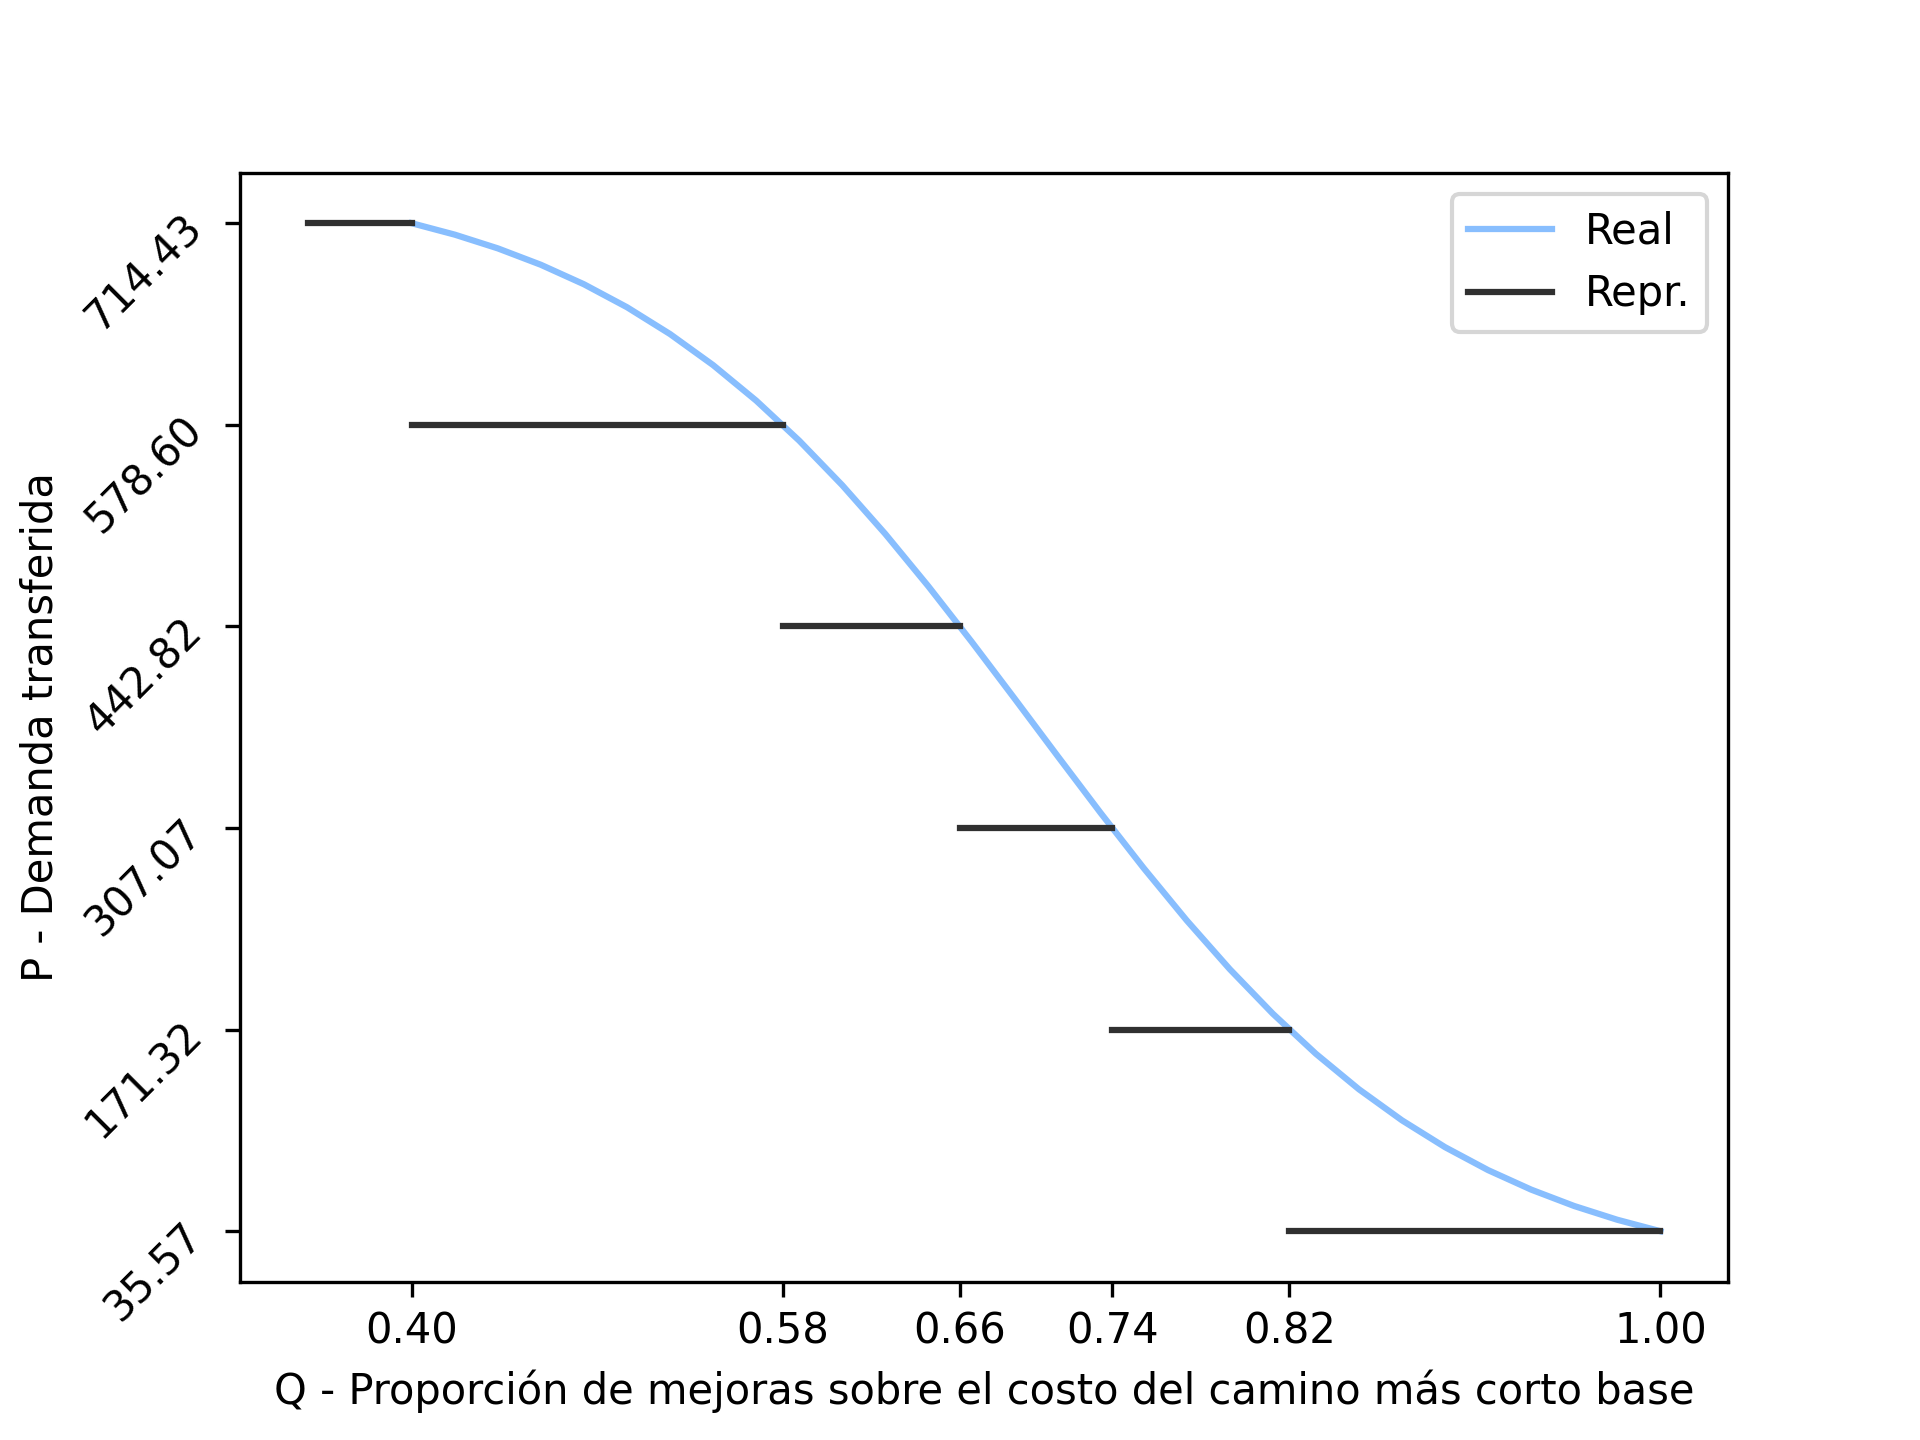
\includegraphics[width=8cm]{../resources/f_example.png}
  \caption{Ejemplo de una función arbitraria y su representación con el mecanismo planteado sobre una demanda total de 750 y un costo del camino más corto base de 1000. Los puntos donde hacer los quiebres son arbitrarios.}
  \label{fig:fdrawexample}
\end{figure}

Una alternativa más precisa de esta representación es la definida en \cite{Crainic2021} donde se presenta un marco para modelar funciones arbitrarias como funciones lineal de a partes con valores de pendiente no nulos entre puntos de quiebre. Esta representación es una generalizacón de la presentada en nuestro trabajo y permite representar de manera más precisa la función real al costo de mayor complejidad al momento de modelarla como problema de programación lineal (LP). Según los autores, debido a la cantidad de variables y restricciones que se agregan con este método es recomendable utilizar algorítmos especializados como Dantzig-Wolfe.

\FloatBarrier
\subsection{Formulación como problema de programación lineal}

La forma más simple de modelar $f_k$ (ó simplemente $f$) es la denotada por (\ref{eq:fkv1eq1})-(\ref{eq:fkv1eq4}). Sea $W \in \mathbb{R}^+$ un valor del costo de un camino:

\begin{align}
  f(W) =\; & max \sum_{j \in J} P_j y_j    & \label{eq:fkv1eq1} \\
           & s.t. \sum_{j \in J} y_j = 1   & \label{eq:fkv1eq2} \\
           & \;\;\; Q_j \geq W y_j         & \label{eq:fkv1eq3} \forall j \in J \\
           & \;\;\; y_j \in \{0,1\}        & \label{eq:fkv1eq4} \forall j \in J
\end{align}

El valor óptimo de esta formulación es el máximo valor $P_j \;|\; Q_j \geq W, j \in J$. La restricción (\ref{eq:fkv1eq3}) deja afuera los valores de $j \in J$ que no cumplen $Q_j \geq W$. Luego, como un único valor de $y_j$ puede estar activo se selecciona aquel que induce el valor máximo de $P_j$ dado que este último esta en el objetivo. Sin embargo, esta formulación no puede ser integrada tal cual está a la formulación (\ref{eq:objectivealt})-(\ref{eq:flowbalancealt}) sin perder linealidad dado que en la última $W$ es modelado con una variable ($w_k$) entonces el resultado seria un problema no lineal por la restricción (\ref{eq:fkv1eq3}). Por este motivo estudiamos dos formulaciones alternativas que logran solucionar esta situación. La idea en ambas es desagregar $W$ como la suma de nuevas variables y utilizar estas en la restricción (\ref{eq:fkv1eq3}) en lugar del producto $W y_j$.

\paragraph*{$f_k$ como LP versión 1}

\begin{align}
  f(W) =\; & max \sum_{j \in J} P_j y_j             & \label{eq:fkv3eq1}\\
           & s.t. \sum_{j \in J} y_j = 1            & \label{eq:fkv3eq2}\\
           & \;\;\; Q_j \geq w^{aux}_j              & \forall j \in J \label{eq:fkv3eq3} \\
           & \;\;\; w^{aux}_j \leq M y_j            & \forall j \in J \label{eq:fkv3eq4} \\
           & \;\;\; w^{sink}_j \leq M (1 - y_j)     & \forall j \in J \label{eq:fkv3eq5} \\
           & \;\;\; w^{sink}_j + w^{aux}_j = W      & \label{eq:fkv3eq6} \forall j \in J\\
           & \;\;\; y_j \in \{0,1\}                 & \label{eq:fkv3domainy} \forall j \in J \\
           & \;\;\; w^{aux}_j, w^{sink}_j \geq 0    & \label{eq:fkv3eq7} \forall j \in J
\end{align}

Se desagrega $W$ para cada $j$ en $w^{sink}_j + w^{aux}_j$ de manera que uno de los dos tenga el valor de $W$, esto se logra con las restricciones (\ref{eq:fkv3eq4}) y (\ref{eq:fkv3eq5}). Entonces se cumple que solo el $w^{aux}_j$ cuyo $y_j$ esté activo tendrá el valor de $W$, mientras que para el resto de los $j$ las variables $w^{sink}_j$ habrán tomado dicho valor. Las mencionadas restricciones sirven para activar $y_i$ y utilizan un parámetro $M \geq W$ arbitrario. Finalmente, las restricciones (\ref{eq:fkv3eq2}) y (\ref{eq:fkv3eq6}) logran que solo una de las variables $w^{aux}_j$ o $w^{sink}_j$ tome el valor de $W$, para cada $j$. Las variables $w^{sink}_j$ sirven para absorber el valor de $W$ cuando $y_j$ está inactiva de manera que se pueda cumplir la restricción (\ref{eq:fkv3eq3}) cuando $W$ es mayor a a $Q_j$.

\paragraph*{$f_k$ como LP versión 2}

\begin{align}
  f(W) =\; & max \sum_{j \in J} P_j y_j             & \label{eq:fkv2eq1}\\
           & s.t. \sum_{j \in J} y_j = 1            & \label{eq:fkv2eq2}\\
           & \;\;\; Q_j \geq w^{aux}_j              & \forall j \in J \label{eq:implfkoriginalineq} \\
           & \;\;\; w^{aux}_j \leq M y_j            & \forall j \in J \label{eq:yactivation1} \\
           & \;\;\; \sum_{j \in J} w^{aux}_j = W    & \label{eq:activatewaux} \\
           & \;\;\; y_j \in \{0,1\}                 & \label{eq:fkv2domainy} \forall j \in J\\
           & \;\;\; w^{aux}_j \geq 0                & \label{eq:fkv2eq6} \forall j \in J
\end{align}

En este caso se desagrega $W$ como suma de $|J|$ variables $w^{aux}_j$ de manera que solo una de ellas esté activa y tenga el valor de $W$. Para activar $y_j$ se agrega la restricción (\ref{eq:yactivation1}) utilizando, igual que en la formulación anterior, un parámetro $M \geq W$. Finalmente, las restricciones (\ref{eq:fkv2eq2}) y (\ref{eq:activatewaux}) logran que solo uno de los $w^{aux}_j$ tome el valor de $W$ y el resto sean 0.

\subsection{Discusión de las formulaciones de transferencia de demanda}

Según definimos $f_k(W)$ en (\ref{eq:deffks}), sea $p = f_k(W)$, entonces se cumple que:

\begin{enumerate}
  \item {\label{deffpt1} $p$ es exactamente uno de los valores del conjunto de valores $P_j$, es decir: $p \in \{P_j\}_{j \in J}$}
  \item {\label{deffpt2} Sea $\hat{j} = j \;|\; p = P_j$. Se cumple que el valor del punto de quiebre $Q$ asociado a $\hat{j}$ no es menor que el costo del camino más corto $W$, es decir: $Q_{\hat{j}} \geq W$.}
  \item {\label{deffpt3} Dado el $\hat{j}$ anterior, entonces no existe un punto de quiebre $Q_j \; \forall j \in J\setminus\{\hat{j}\}$ que sea no mayor al punto de quiebre $Q_{\hat{j}}$ y mayor o igual al costo del camino más corto, es decir: $\not{\exists}\; Q_j\; \forall j \in J\setminus\{\hat{j}\} \;|\; Q_j \in  [W, Q_{\hat{j}}]$}.
\end{enumerate}

Es de nuestro interés analizar la correctitud de las formulaciones respecto a los puntos mencionados. Para la versión 1, tenemos que el punto \ref{deffpt1} se cumple en la función objetivo donde se establece el valor objetivo como la suma sobre el conjunto $\{P_j\}_{j \in J}$, la restricción (\ref{eq:fkv3eq2}) dice que solo uno de esos valores puede estar activo en la suma del objetivo dado el dominio de la variable $y_j$. Luego, el punto \ref{deffpt2} se cumple dado que $y_{\hat{j}} = 1$ por el punto anterior, entonces $w_{\hat{j}}^{aux} = W$ por restricciones (\ref{eq:fkv3eq4}), (\ref{eq:fkv3eq5}) y (\ref{eq:fkv3eq6}) y la restricción (\ref{eq:fkv3eq3}) verifica el punto en cuestión. Finalmente, el punto \ref{deffpt3} se cumple por el hecho de que la función objetivo es una maximización y que $f(W)$ es una función estrictamente decreciente, entonces, si existiera un $Q_a \in \{Q_j\}_{j \in J} \;|\; Q_a < Q_{\hat{j}} \;\text{y}\; Q_a \geq W, a \in J$, existe un valor $P_a > P_{\hat{j}}$ lo que contradice el hecho de que el objetivo sea una maximización.

Podemos utilizar las justificaciones de los puntos 1 y 3 para la versión 2 de la formulación. Luego, el punto \ref{deffpt2} se cumple dado que $y_{\hat{j}} = 1$ por los puntos anteriores y considerando que $w^{aux}_{\hat{j}} = W$ por las restricciones (\ref{eq:fkv2eq2}), (\ref{eq:yactivation1}) y (\ref{eq:activatewaux}) tenemos que la condición se cumple en la restricción (\ref{eq:implfkoriginalineq}).

\subsection{Valores posibles de $P_j$ y $Q_j$}

Los valores que tienen sentido para los conjuntos $Q$ y $P$ son cualquier subconjunto discreto del dominio de la función de transferencia de demanda y su valor funcional, respectivamente. Dada una instancia del problema y un par origen destino $k$, llamamos $\underline{W}$ al costo del camino más corto suponiendo que las mejores tecnologías se pueden construir y $\overline{W}$ al costo del camino más corto sobre el grafo base (sin infraestructura de ciclovía especializada) \footnote{En realidad, $\overline{W}$ es el mínimo valor para el que $f_k$ es mínimo, podría ser cualquier número arbitrariamente grande.}, entonces $Q_j \in [\underline{W}, \overline{W}],\; \forall j \in J$. Los valores de $Pj$ son la cantidad de demanda que se transfiere para cada $Q_j$, es decir $P = \{f_k(Q_j):\; j \in J\}$. El conjunto índice $J$ determina la precisión con que se representa la función $f_k$ y el órden en que define los puntos de quiebre es el siguiente: sea $J = \{1, 2, .. , J_{max}\}$ entonces $P_j < P_{j+1}$ y $Q_j > Q_{j+1}$, es decir, a mayor valor del índice $j$ mayor es el valor de demanda transferida y mejor es el camino para el usuario.

Además, entendemos que tiene sentido que el dominio de $f_k$ sean valores de costos de usuario de camino más cortos que van desde aquel para el cual toda la demanda se transfiere hasta aquel para el cual no hay demanda transferida. Es decir, que el mínimo de $f_k$ sea 0 y que el máximo sea la demanda total del par $k$: $d_k$, osea $f_k(\overline{W}) = 0$ y $f_k(\underline{W}) = d_k$. Esto quiere decir que si no hay infraestructura de ciclovias o la infraestructura construida no afecta el costo del camino más corto entonces no debe haber transferencia de demanda. Por otro lado, si la mejor tecnología posible es construida de manera que el costo del camino más corto disminuya a $\underline{W}$ entonces toda la demanda se transfiere. Lo anterior es consistente con la hipótesis de que trabajamos exclusivamente con la demanda transferible a la bicicleta dejando afuera la que ya utiliza dicho medio de transporte, la que en ningún caso la utilizaría y la que requiere de costos de usuario demasiado bajos para las posibilidades de la instancia. Por lo tanto, en la definición una función $f_k, k \in OD$ tienen relevancia aspectos como el grafo base y el costo del camino más corto sobre él para el par origen-destino $k$ y las tecnologías de ciclovias que pueden ser construidas y cómo afectan al costo de usuario al ser activadas.

Una forma posible de establecer los valores de $J$, $P_j$ y $Q_J$ es: dada una función $f_k$, tomando $N$ valores equidistantes entre $[\underline{W}, \overline{W}]$ obtendremos $Q_j$ y tomando el valor funcional de esos puntos obtendremos $P_j$, luego $J=\{1,..,N\}$.

\section{Formulación integrada}
\label{sect:alltogether}

Luego del análisis hecho en las secciones \ref{sect:variableproductremoval}, \ref{sect:singlelevelformulation} y \ref{sect:transferfunctiondefs}, ensamblamos la formulación MILP de un nivel de manera explícita. Dado que tenemos dos variantes del modelado de las funciones de transferencia de demanda entonces también tendremos dos variantes de esta formulación. Aquí presentamos la formulación completa utilizando la versión 2 de $f_k$, siendo la otra muy similar. Fundamentalmente sobre estas dos variantes trabajamos en lo que sigue.

Además de las definiciones en la formulación inicial (\ref{eq:objective1lvl})-(\ref{eq:flowbalance}), agregamos las siguientes:

\begin{description}
  \item[$J$]: Conjunto índice utilizado en los conjuntos $P$ y $Q$.
  \item[$P_{kj}$]: Parámetro que determina la cantidad de demanda transferida para el par origen-destino $k \in OD$ y el índice $j \in J$.
  \item[$Q_{kj}$]: Parámetro que contiene el punto de quiebre para determinar la demanda transferida para el par origen-destino $k \in OD$ e índice $j \in J$.
  \item[$M$]: Número positivo muy grande.
  \item[$z_{kj}$]: Variable binaria que determina si la demanda transferida para el par origen-destino $k \in OD$ es la de índice $j \in J$.
  \item[$h_{aki}$]: Variable no negativa que determina el flujo que pasa por el arco $a \in A$, para el par origen-destino $k \in OD$ utilizando la tecnología $i \in I$.
  \item[$w^{aux}_{kj}$]: Variable no negativa que contiene el valor de $w_{k}$ si $z_{kj}$ está activa y de lo contrario cero.
\end{description}

La formulación que resulta de la integración de las formulaciones (\ref{eq:objectivealt})-(\ref{eq:flowbalancealt}) que define la formulación de un nivel, de (\ref{eq:subproblemrefeq1})-(\ref{eq:subproblemrefeq4}) que quita el producto de variables y de (\ref{eq:fkv2eq1})-(\ref{eq:fkv2eq6}) que define la versión 2 de las funciones de transferencia de demanda es la siguiente:

\begin{align}
  \text{max}    & \sum_{k \in OD} \sum_{j \in J} P_{kj} z_{kj}                          & \label{eq:objectivefinalalt} \\
  \text{s.t.}\; & w_k = \sum_{a \in A} \sum_{i \in I} C_{ai}h_{aki}                     & \forall k \in OD \label{eq:shortestpathaltfinal} \\
                & Q_{kj} \geq w^{aux}_{kj}                                              & \forall j \in J, k \in OD \label{eq:breakpointsalt} \\
                & w^{aux}_{kj} \leq M z_{kj}                                            & \forall j \in J, k \in OD \\
                & \sum_{j \in J} w^{aux}_{kj} = w_k                                     & \forall k \in OD \\
                & \sum_{j \in J} z_{kj} = 1                                             & \forall k \in OD \label{eq:singularbreakpointalt} \\
                & B \geq \sum_{a \in A} \sum_{i \in I} H_{ai}y_{ai}                     & \label{eq:respectbudgetaltfinal} \\
                & 1 = \sum_{i \in I} y_{ai}                                             & \forall a \in A \label{eq:alwaysoneyaltfinal} \\
                & \sum_{a \in A_n^+} x_{ak} - \sum_{a \in A_n^-} x_{ak} = \theta_{nk}   & \forall n \in N, k \in OD \label{eq:flowbalancealtfinal} \\
                & x_{ak} = \sum_{i \in I} h_{aki}                                       & \forall a \in A, k \in K \label{eq:flowactivationalt} \\
                & 0 \leq h_{aki} \leq y_{ai}                                            & \forall a \in A, k \in K, i \in I \label{eq:respectinfraalt} \\
                & z_{kj} \in \{0,1\}                                                    & \forall k \in OD, j \in J \nonumber \\
                & y_{ai} \in \{0,1\}                                                    & \forall a \in A, i \in I \nonumber \\
                & h_{aki} \geq 0                                                        & \forall a \in A, k \in K, i \in I \nonumber
\end{align}

Donde las nuevas ecuaciones son:

\begin{description}
  \item[\ref{eq:objectivefinalalt}]: Función que suma los valores de demanda transferida $P_{kj}$ correspondiente a los puntos de quiebre activos.
  \item[\ref{eq:breakpointsalt}]: Restricción que determina que los puntos de quiebre activos, son aquellos cuyo costo es menor o igual al del camino más corto.
  \item[\ref{eq:singularbreakpointalt}]: Restricción que permite solo un punto de quiebre activo para cada par origen-destino $k \in OD$.
  \item[\ref{eq:flowactivationalt}]: Restricción que fija el valor del flujo por arco por par origen-destino en base al flujo por arco, par origen-destino y tecnología.
  \item[\ref{eq:respectinfraalt}]: Restricción que limita el flujo desagregado por arco y tecnología ($h_{aki}$) a la tecnología activa en el arco. El flujo por el arco $a \in A$, para el par origen-destino $k \in OD$ y la tecnología $i \in I$ puede estar activo si la tecnología $i$ esta activa.
\end{description}

\section{Análisis de la formulación}

En esta sección analizamos las dos variantes de la formulación de un nivel (\ref{eq:objectivefinalalt})-(\ref{eq:respectinfraalt}) con pequeñas variantes adicionales y mostramos su validez de manera experimental.

Como mecanismo de validación, utilizamos las características que debe cumplir una solución mencionadas al principio en la sección \ref{sect:solutioncharacteristics}, página \pageref{sect:solutioncharacteristics}. Comprobando dichos puntos sobre las soluciones obtenidas por las formulaciones estudiadas podemos tener confianza de que ellas resuelven lo deseado. También fueron de utilidad verificar la implementación computacional durante su desarrollo.

% \subsection{Variantes de la formulación}

Durante la implementación y pruebas preliminares de la formulación (\ref{eq:objectivefinalalt})-(\ref{eq:respectinfraalt}) observamos que en algunos casos los flujos no eran consistentes con la hipótesis del comportamiento de los usuarios, es decir, no iban por el camino más corto entre origen y destino. La explicación es que las funciones $f_k$ son constantes entre dos valores consecutivos de $Q_{kj}$ lo cual causa que en dicho dominio no exista incentivo para optimizar el costo del camino más corto. Para corregir esto consideramos dos opciones, que en definitiva cambian nuestra formulación de un objetivo único a una multiobjetivo jerárquico donde el objetivo primario sigue siendo el de maximizar la demanda transferida total (\ref{eq:objectivefinalalt}) y el secundario se presenta a continuación.

En la primera opción agregamos variables de holgura $r_{kj} \geq 0$ que modelan la diferencia entre el punto de quiebre $Q_{kj}$ activo y el costo del camino más corto $w_k$ para un par origen-destino. Dichas variables también son agregadas a la función objetivo como objetivo secundario. Esto cambia el modelado de las funciones $f_k$ en la ecuación (\ref{eq:breakpointsalt}) que queda de la siguiente manera:

\begin{equation}
  \label{eq:multipleobj1breakpoint}
  Q_{kj} z_{kj} - r_{kj} = w^{aux}_{kj}
\end{equation}

Advertir que esta restricción se encuentra en ambas versiones de la formulaciones de $f_k$ por lo tanto en ambos casos se aplica esta variante.

Luego, sea el parámetro $\beta \geq 0$, la función multiobjetivo 1 es:

\begin{equation}
  \label{eq:multipleobj1}
  \sum_{k \in OD} \sum_{j \in J} \left( P_{kj}z_{kj} + \beta r_{kj} \right)
\end{equation}

Otra forma de abordar esta situación es vincular los objetivos de los problemas de primer y segundo nivel en (\ref{eq:objective1lvl})-(\ref{eq:flowbalance}). Dado que los dos objetivos optimizan en direcciones contrarias entonces el coeficiente del objetivo secundario, que originalmente era una minimización, necesita ser un valor negativo. Sea el parámetro $\rho \geq 0$, entonces podemos expresar la función multiobjetivo 2 como:

\begin{equation}
  \label{eq:multipleobj2}
  \sum_{k \in OD} \left[ -\rho w_k + \sum_{j \in J} P_{jk}z_{kj} \right]
\end{equation}

Notar que al modificar el objetivo del problema estamos, estrictamente hablando, solucionando otro problema. Sin embargo a los efectos prácticos podemos en este caso encontrar valores de los pesos relativos de cada objetivo secundario de manera de que se resuelva correctamente nuestro problema y se pueda calcular la demanda transferida total con posterioridad a la resolución. Dicho de otra manera, para cada peso $\beta$ y $\rho$ existe un intervalo $[0, \beta_{max}]$ y $[0, \rho_{max}]$ respectivamente, en el que el valor computado de demanda transferida es igual. Tenemos diferentes interpretaciones para cada objetivo secundario. En el caso del multiobjetivo 1, dado que la dirección de optimización es la misma que el objetivo primario, lo que tiene que suceder, intuitivamente, es que el valor del objetivo secundario sea intrascendente respecto a los saltos posibles en los puntos de quiebre para cada par origen destino lo que permite que ambos objetivos puedan comportarse de manera independiente. En el caso del multiobjetivo 2, dado que el objetivo secundario optimiza en dirección contraria al primario, no hay límites en el valor máximo de $\rho$ por lo que diremos que $\rho_{max} > 0$.

Otra desventaja de modificar el objetivo, en particular en problemas MILP con instancias difíciles, es que perdemos capacidad de interpretación del MILP GAP, o distancia relativa de la mejor solución factible a la mejor cota encontradas por el solver hasta cierto punto de la ejecución del algorítmico Branch and Bound, dado que el valor objetivo es una suma de unidades potencialmente distintas.

\subsection{Ejemplo - Comparativa de variantes de un objetivo y multiobjetivo}
\label{sect:example2}

Este ejemplo busca ilustrar por qué es necesario agregar nuevos objetivos a la función objetivo de (\ref{eq:objectivefinalalt})-(\ref{eq:respectinfraalt}) de forma de optimizar no solo la demanda transferida, sino que también obtener una buena decisión de ubicación y tipo de tecnología.

Para este ejemplo utilizaremos como base la red descrita en la Tabla \ref{table:example2arccosts} y en la Figura \ref{fig:example2base}. Al igual que el ejemplo presentado en la sección \ref{sect:example1}, consideramos el costo de usuario sobre la tecnología base y el costo de construcción de la primer tecnología no base como el costo de los arcos que se detallan en dicha figura. Consideramos solo dos tipos de tecnologías, la base y la tecnología 1 que reduce el costo de usuario a la mitad; un par origen-destino, $(1, 6)$ con demanda $D$, un presupuesto de 5 y la siguiente función de transferencia de demanda:

$$
  f(x) = \left\{ \begin{array}{lcr}
          D & \mbox{si}   & x \leq 4.5 \\
          0 & \mbox{sino} &
        \end{array}
        \right.
$$

\begin{table}[h!]
  \centering
  \begin{tabular}{cccccc}
    \toprule
    Arco & CU base & CU 1 & CC base & CC 1 & \\
    \midrule
      (1, 2) & 3 & 1.5 & 0 & 3 \\
      (1, 3) & 3 & 1.5 & 0 & 3 \\
      (1, 5) & 4 & 2   & 0 & 4 \\
      (2, 3) & 2 & 1   & 0 & 2 \\
      (2, 4) & 3 & 1.5 & 0 & 3 \\
      (3, 2) & 3 & 1.5 & 0 & 3 \\
      (3, 4) & 2 & 1   & 0 & 2 \\
      (3, 5) & 2 & 1   & 0 & 2 \\
      (4, 5) & 4 & 2   & 0 & 4 \\
      (4, 6) & 2 & 1   & 0 & 2 \\
      (5, 4) & 4 & 2   & 0 & 4 \\
      (5, 6) & 2 & 1   & 0 & 2 \\
    \bottomrule
  \end{tabular}
    \caption{Resumen de costos de usuario (CU) y de construcción (CC) para cada tecnología de ciclovía.}\label{table:example2arccosts}
\end{table}

\begin{figure}[h!]
  \centering
  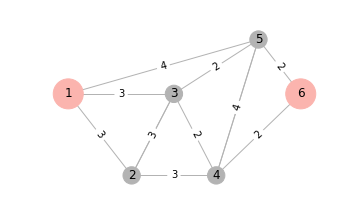
\includegraphics[width=6cm]{../resources/example_2_base.png}
  \caption{Red utilizada para el ejemplo de beneficio de variantes multiobjetivo. El camino más corto sobre el grafo base es el (1, 5), (5, 6) de costo 6.}
  \label{fig:example2base}
\end{figure}

\FloatBarrier

Presentamos dos soluciones: la S utilizando la variante de un único objetivo (\ref{eq:objectivefinalalt})-(\ref{eq:respectinfraalt}) y la SM utilizando cualquiera de las variantes multiobjetivo (ecuaciones (\ref{eq:multipleobj1}) ó (\ref{eq:multipleobj2})).

La solución S, representada en la Figura \ref{fig:example2solv2}, tiene las siguientes características:

\begin{itemize}
  \item{Demanda transferida total: $D$}
  \item{Tecnología de tipo 1 construida en arcos (1, 3) y (4, 6)}
  \item{Presupuesto utilizado: 5}
  \item{El camino más corto es (1, 3), (3, 4), (4, 6) con costo 4.5}
\end{itemize}

Mientras que la solución SM, en la Figura \ref{fig:example2solv1}:

\begin{itemize}
  \item{Demanda transferida total: $D$}
  \item{Tecnología de tipo 1 construida en el arco (1, 5)}
  \item{Presupuesto utilizado: 4}
  \item{El camino más corto es (1, 5), (5, 6) con costo 4}
\end{itemize}

Las decisiones tomadas por la versión multiobjetivo fueron mejores en términos de la infraestructura de ciclovía a construir que la de un único objetivo ya que el costo de usuario resultante disminuyó en mayor cantidad y el presupuesto utilizado fue menor, aunque esto último es circunstancial. Para analizar el porqué primero debemos definir los puntos de quiebre de esta instancia. Dada la simplicidad de la función de transferencia de demanda podemos utilizar solo dos puntos de quiebre, entonces $J = \{0, 1\}$, $Q = \{6, 4.5\}$ y $P = \{0, D\}$. Omitiremos los índices $k$ del par origen-destino dado que existe uno solo. Tenemos que el $z_j$ activo, que determina el valor de demanda transferida, es aquel con $j = 1$ dado que sabemos que la demanda transferida es $D$.

Considerando la opción multiobjetivo 1 (\ref{eq:multipleobj1}), tenemos de la restricción (\ref{eq:multipleobj1breakpoint}) que $r_1 = Q_1 - w^{aux}$ y siendo $w^{aux} = w$ por ser el punto de quiebre activo entonces $r_1 = 4.5 - w$ y el valor objetivo es $D + r_1$. Aplicando las soluciones a estas ecuaciones tenemos que para la solución S $r_1 = 0$ y para SM $r_1 = 0.5$. Por lo tanto la presencia de $r_{kj}$ en el objetivo ayuda a elegir la solución SM sobre la S en este caso.

Si utilizamos la formulación multiobjetivo 2 (\ref{eq:multipleobj2}), tenemos que el valor objetivo evaluado en la solución S es $D - 4.5$ y en la solución SM es de $D - 4$, por lo tanto la solución SM también es mejor según esta formulación.

Vale la pena aclarar que las solución SM es, para la versión de un único objetivo, tan buena como la S. En general, asumiendo que los pesos $\beta$ y $\rho$ fueron elegidos de acuerdo a la sección anterior, las soluciones obtenidas por las versiones multiobjetivo también son soluciones óptimas de la de un único objetivo.

Finalizamos este ejemplo comentando que ambas soluciones S y SM satisfacen los criterios definidos en las características de una solución definidas en la sección (\ref{sect:solutioncharacteristics}), página \pageref{sect:solutioncharacteristics}.

\begin{figure}[h!]
  \centering
  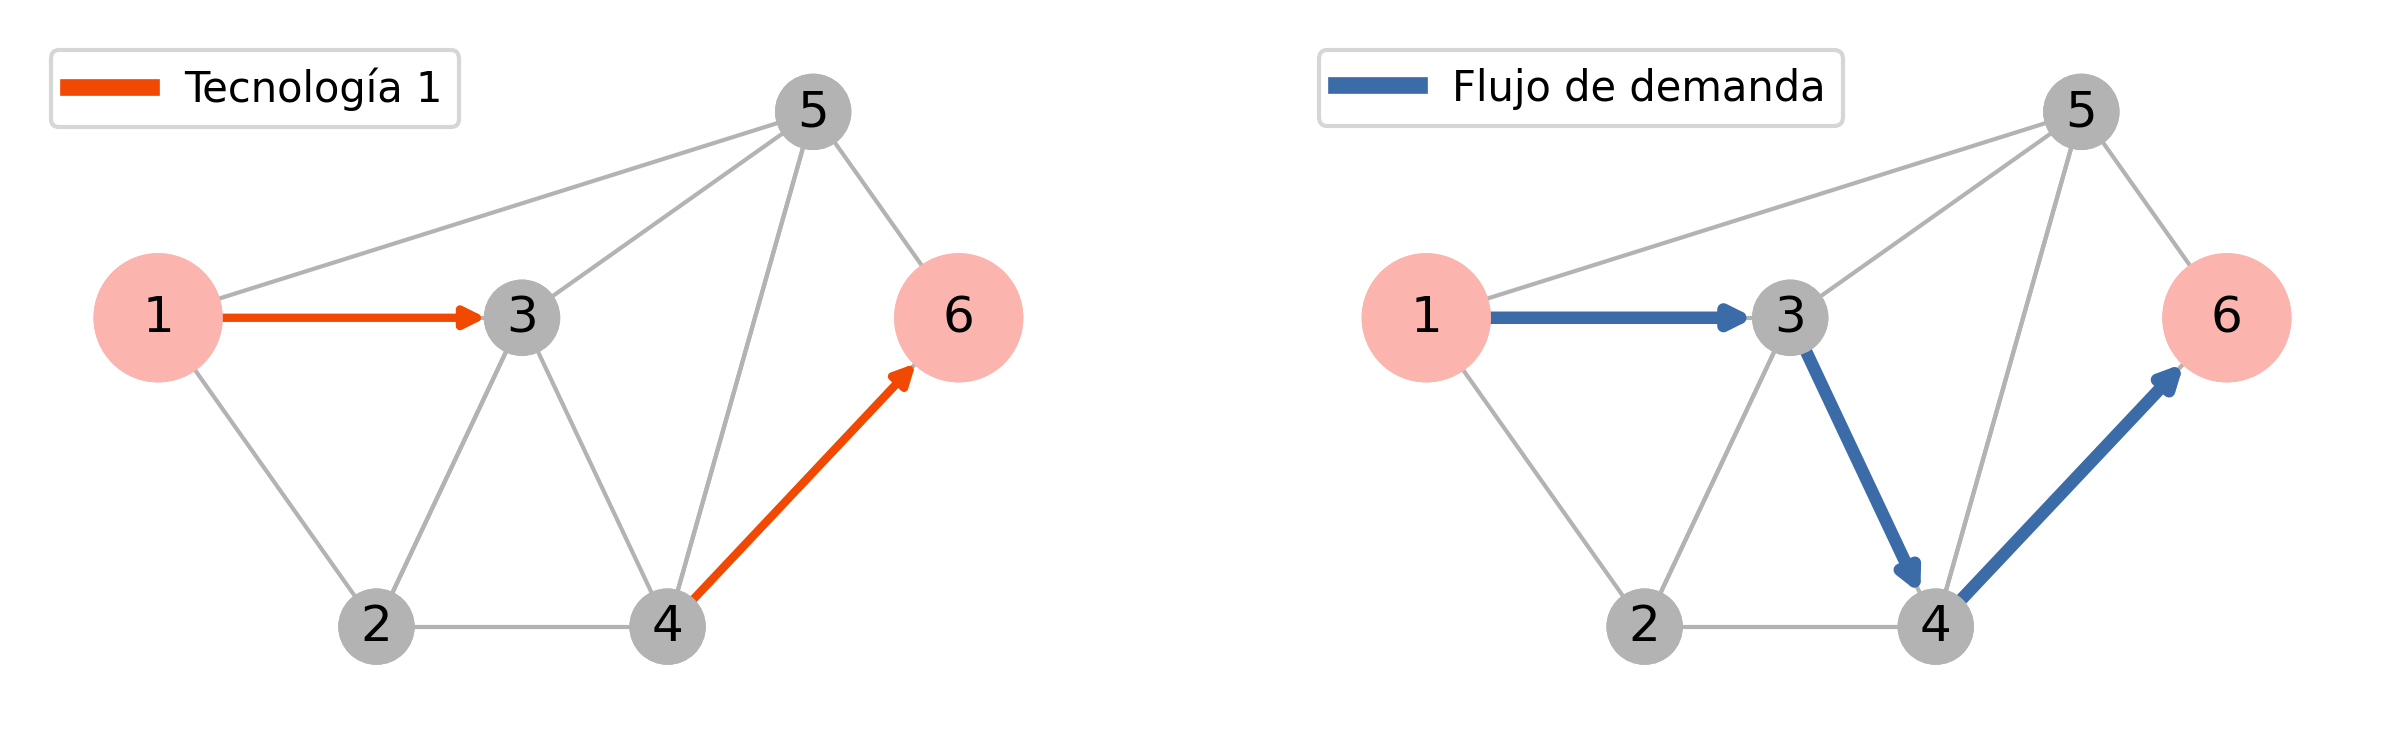
\includegraphics[width=12cm]{../resources/example_2_sol_v2.png}
  \caption{Representación de la solución S. A la izquierda se resaltan los arcos donde se construye la tecnología 1. A la derecha se observa el camino más corto sobre la red resultante.}
  \label{fig:example2solv2}
\end{figure}

\begin{figure}[h!]
  \centering
  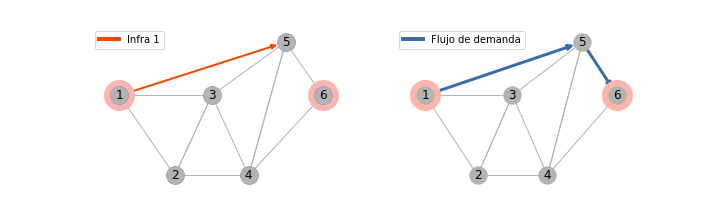
\includegraphics[width=12cm]{../resources/example_2_sol_v1.png}
  \caption{Solución SM. A la izquierda se resalta el arco donde se construye la tecnología 1 mientras que a la derecha se muestra el camino más corto, que coincide con el de la red base.}
  \label{fig:example2solv1}
\end{figure}

\FloatBarrier
\section{Análisis experimental}

El procedimiento de validación experimental consistió en generar instancias aleatorias, solucionarlas con las diferentes versiones y verificar que se cumplan las condiciones sobre las soluciones. Las diferentes alternativas fueron sobre la formulación de un nivel, dadas por las dos implementaciones de las $f_k$, las dos versiones multiobjetivo y la versión de un único objetivo. Consideraremos en principio parámetros $\beta = 1$ y $\rho = 1$ dado que obtuvimos resultados correctos con esta asignación en una ronda de pruebas preliminares.

Utilizamos la instancia de Sioux-Falls como grafo base, dada su amplia adopción en literatura relativa al tema \cite{Liu2019}, datos que dejamos disponibles en el Apéndice \ref{sect:siouxfallsdata}. El costo de usuario de la tecnología base se tomó igual al largo del arco así como el costo de construcción de la primer tecnología no base. Consideramos en total tres tipos de tecnologías incluyendo la base, es decir $I = \{0, 1, 2\}$. El cálculo de costos de usuario y construcción se realizó en base a los costos de usuario base y de construcción para la tecnología 1, como se detalla en el Apéndice \ref{sect:costcalculation}, página \pageref{sect:costcalculation}.

Se generaron entre 1 y 14 pares origen-destino y entre 2 y 10 valores de $P$ y $Q$ aleatorios cumpliendo con la hipótesis de modelar una función decreciente.
De esta manera se generaron y probaron 1000 instancias para cada una de las seis variantes de las formulaciones. Nos interesa verificar si las soluciones cumplen con las características definidas en \ref{sect:solutioncharacteristics}: 1) que el costo de los caminos más cortos sobre la red resultante, es decir con infraestructura de ciclovía, es menor o igual al costo sobre la red sin infraestructura; 2) que el presupuesto excedente no es suficiente para construir infraestructura que mejore el costo del camino más corto de algún par origen-destino; 3) y que el costo del camino más corto sobre la red resultante no induce una demanda transferida distinta de la resultante. Ademas fue de nuestro interés comparar los valores de demanda transferida total y tiempos de ejecución.

\FloatBarrier
\subsection{Resultados}

\begin{table}[h!]
  \centering
  \begin{tabular}{cccccc}
    \toprule
    Versión & Versión $f_k$ & Multiobj. 1 & Multiobj. 2 & \shortstack{Cant. \\ Incump.} & \shortstack{Tiempo \\ Promedio (s)} \\
    \midrule
    v1 & v2 & Si & No & 0   & 9.34    \\
    v2 & v2 & No & No & 76  & 22.94   \\
    v3 & v1 & Si & No & 0   & 539.78  \\
    v4 & v1 & No & No & 67  & 495.80  \\
    v5 & v2 & No & Si & 0   & 11.92   \\
    v6 & v1 & No & Si & 0   & 283.93  \\
    \bottomrule
  \end{tabular}
  \caption{Comparativa agregada de ejecuciones sobre instancias aleatorias utilizando la red Sioux-Falls. Los incumplimientos de una solución fueron contados en 1 si la solución no cumplía al menos uno de los puntos. En las versiones v2 y v4 los incumplimientos detectados incumplen únicamente el punto (\ref{budgetexcess}) de las características de una solución.}\label{table:resumenejecuciones}
\end{table}

En las pruebas no detectamos diferencias en términos de los valores objetivos entre diferentes formulaciones a excepción de una instancia. Para la versión v1 y v3, encontramos que la presencia de variables $r_{kj}$ en el objetivo puede resultar en una solución que induce menor valor de demanda transferida total en comparación a las otras formulaciones cuando se cumple que el valor de demanda transferida para un par origen-destino $k$ es comparable a la magnitud de $r_{kj}$, dado que $z_{kj}$ está activa. Por ejemplo, si para un par origen-destino se puede optimizar el camino más corto de manera de transferir cierta cantidad de demanda adicional pero esto afecta la variable $r_{kj}$ de manera que la diferencia con el siguiente punto de quiebre es mayor que el nuevo salto en demanda transferida, entonces el modelo elige no realizar la mejora.

También observamos que en las versiones v2 y v4, que optimizan un único objetivo, se ve afectada en algunos casos la validez del ítem (\ref{budgetexcess}) de la característica de una solución. Esto se explica en casos en que la construcción de infraestructura en un arco puede mejorar el costo del camino más corto pero no lo suficiente para afectar la cantidad de demanda transferida, lo cual implica que las decisiones de las tecnologías a construir pueda ser peor que en las otras variantes en el sentido del costo del camino más corto, como se mostró en el ejemplo \ref{sect:example2}. A diferencia del ejemplo sin embargo, el presupuesto excedente es suficientemente para mejorar el camino de algún par origen-destino lo que causa el incumplimiento.

A pesar de las diferencia encontrada en el valor de demanda transferida en un caso para las versiones v1 y v3, consideramos que aquellas multiobjetivo son las candidatas a ser elegidas como versión final dado que nos interesa tanto el valor objetivo como las decisiones en términos de la infraestructura ciclovía. Las diferencias en los valores de demanda transferida pueden ser corregidas como se muestra a continuación ajustando el peso $\beta$ del objetivo secundario.

El siguiente aspecto que tuvimos en cuenta es el tiempo de ejecución. El tiempo de ejecución promedio nos da una medida gruesa para comparar y descartar algunas versiones, considerando que las instancias de prueba son chicas y deberían ser de fácil resolución \footnote{El ser fácil está directamente relacionado a la complejidad en tiempo.}. Las versiones v3, v4 y v6, que utilizan la formulación v1 de $f_k$ tienen un tiempo de ejecución promedio significativamente más alto que las demás (Tabla \ref{table:resumenejecuciones}), que utilizan la otra versión. Nos interesó determinar si esta diferencia se da por algún tipo de instancia particular y si alguna versión se desempeña mejor en términos de tiempo de ejecución cuando quitamos las posibles instancias anormales en caso de que existan. En la Figura \ref{fig:runtimecomparison} se puede comparar el tiempo de ejecución de las versiones en todas instancias ejecutadas. Las versiones con mayor tiempo de ejecución promedio (v3, v4 y v6) muestran un peor comportamiento en general en comparación con las otras. También comparamos las dos versiones con menor tiempo promedio de ejecución, donde observamos que la v1 es en la mayoría de los casos la más rápida. Para las instancias más sencillas (primeros tres quintiles de las instancias, ver Figura \ref{fig:firstfourquintiles}), los tiempos de ejecución no varían demasiado entre formulaciones y solo hacia el cuarto quintil se notan diferencias aunque estas son de algunos segundos.

\begin{figure}[h!]
  \centering
  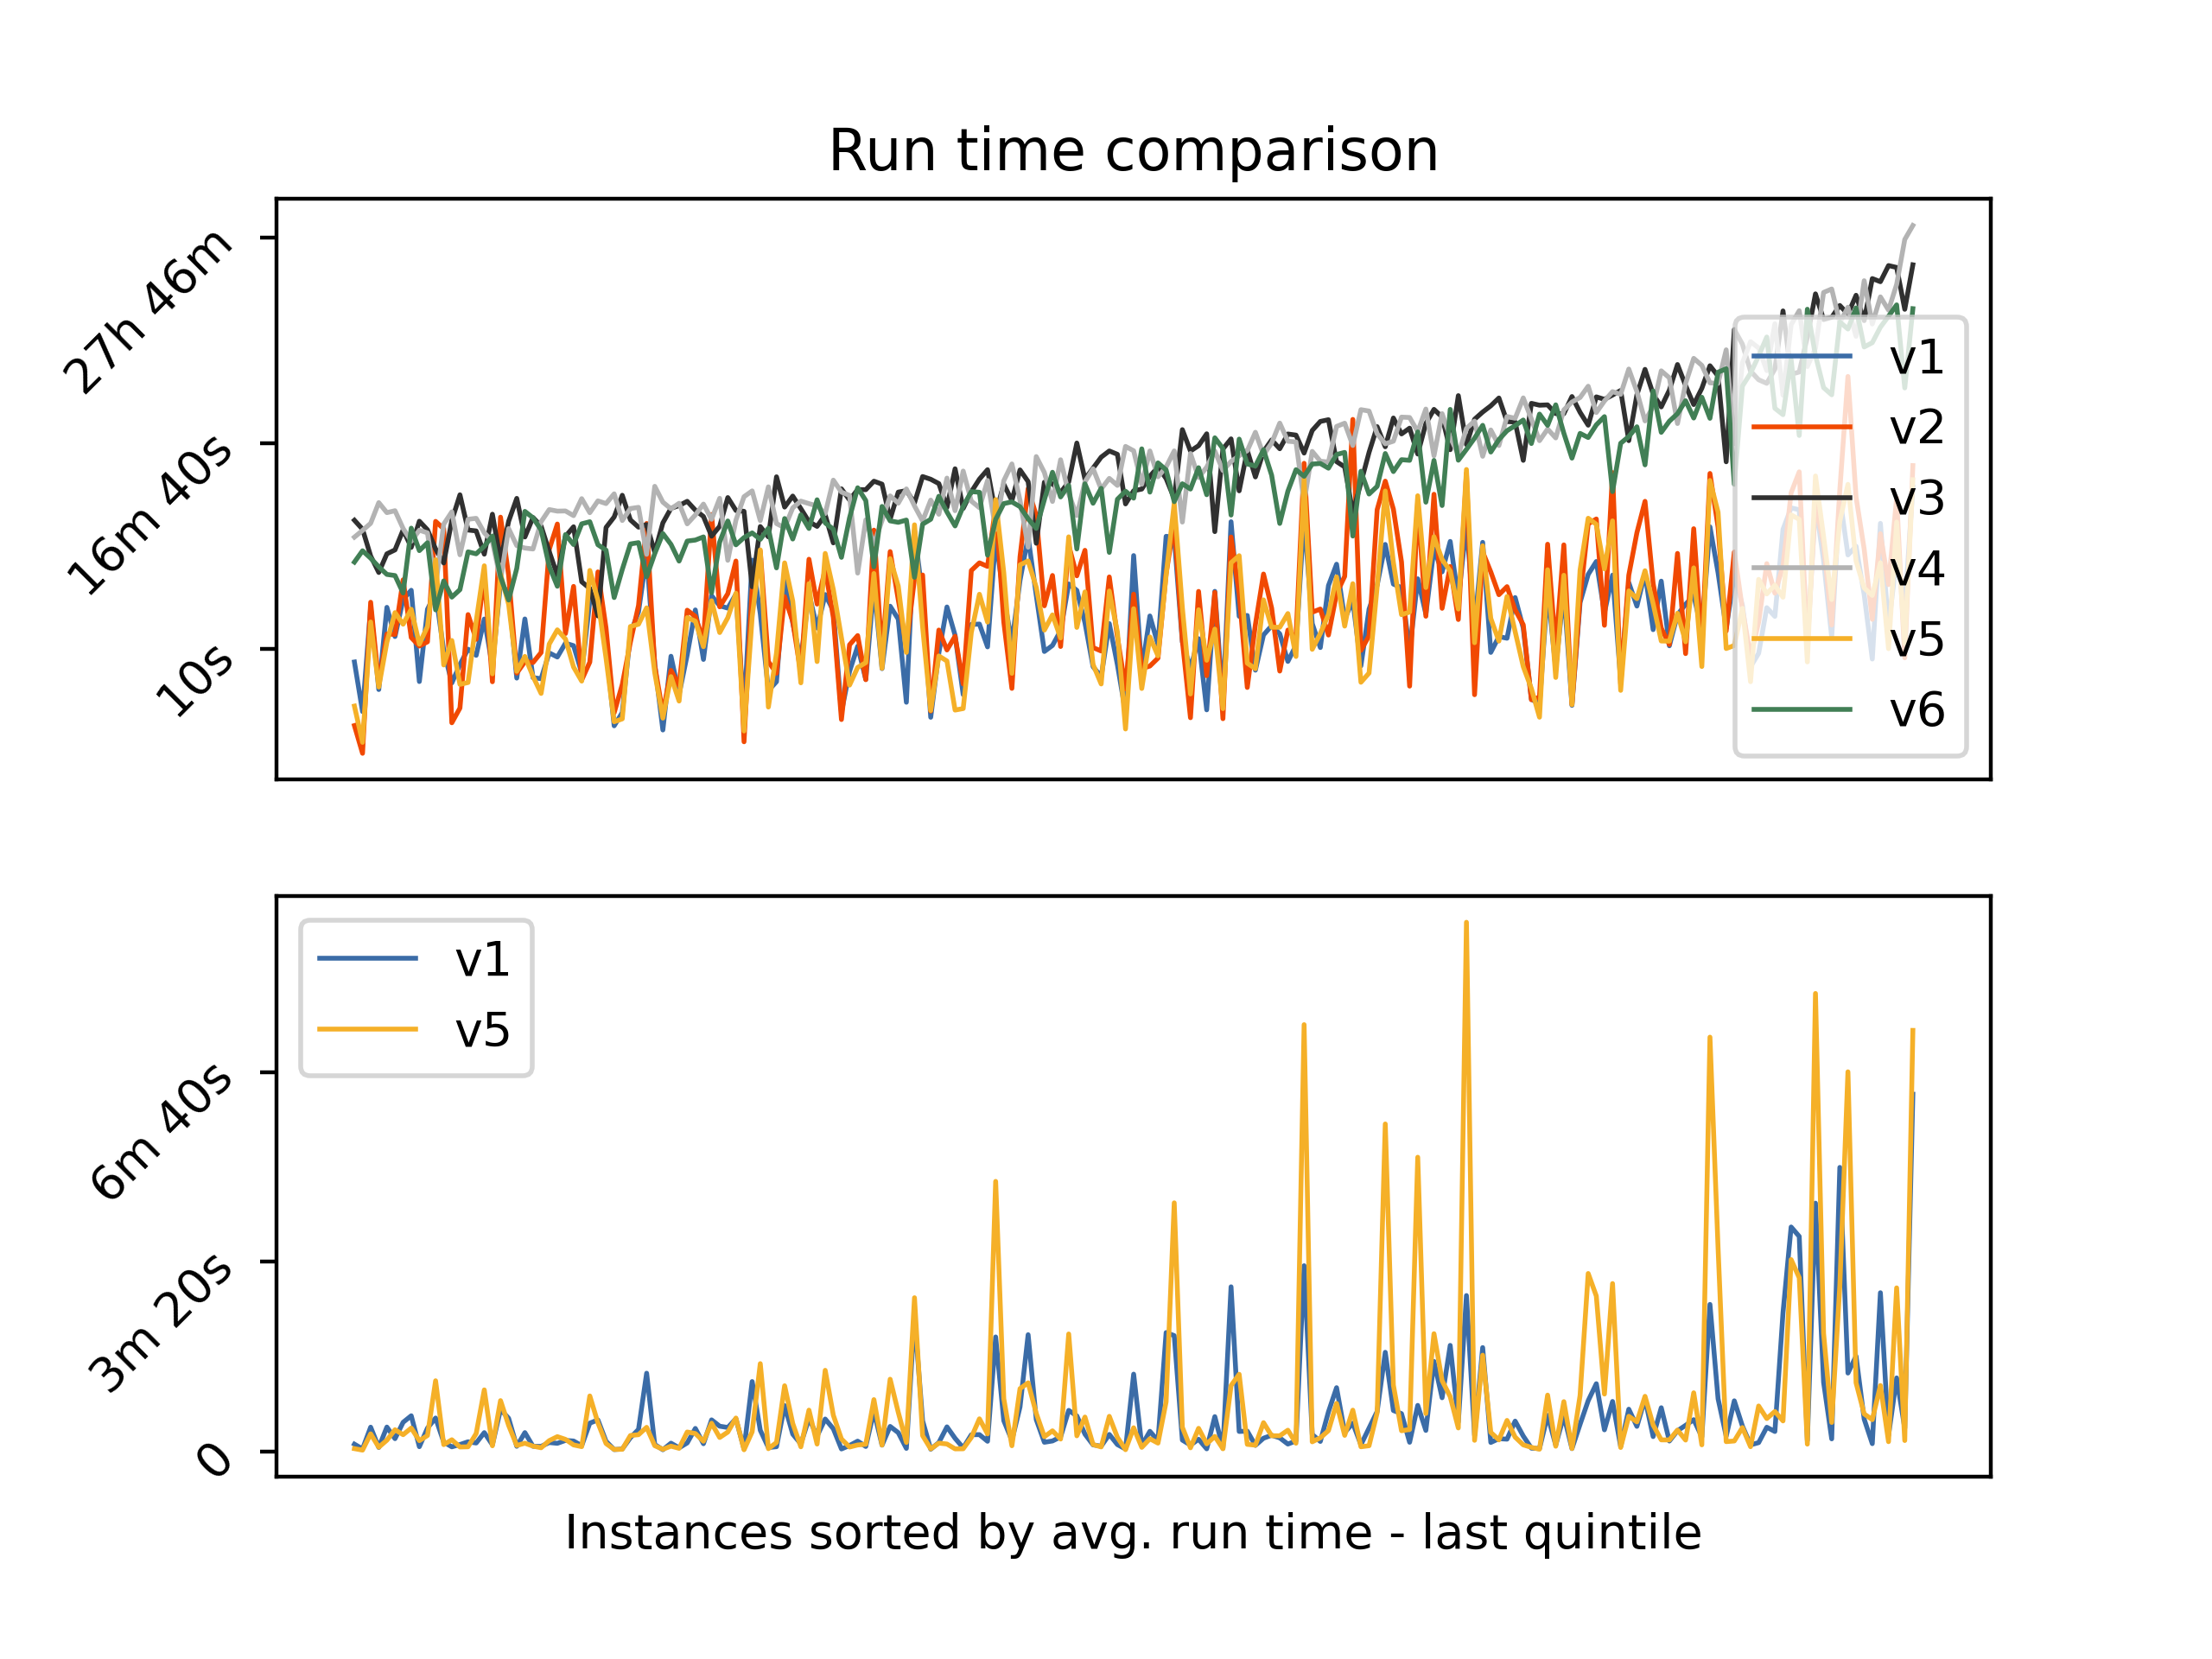
\includegraphics[width=10cm]{../resources/run_time_comparsion.png}
  \caption{Comparativa del tiempo de ejecución de todas las versiones. Las instancias, en las abscisas, fueron ordenadas de forma creciente según el tiempo promedio de ejecución de todas las versiones. En la gráfica superior, la escala es logarítmica, dado que los valores a comparar oscilan entre pocos segundos y casi treinta horas. En la segunda gráfica la escala es lineal, tomamos la última quinta parte de las instancias ordenadas y las dos versiones con menor tiempo de ejecución para mostrar mejor la escasa diferencia entre ellas en las instancias más difíciles.}
  \label{fig:runtimecomparison}
\end{figure}

\begin{figure}[h!]
  \centering
  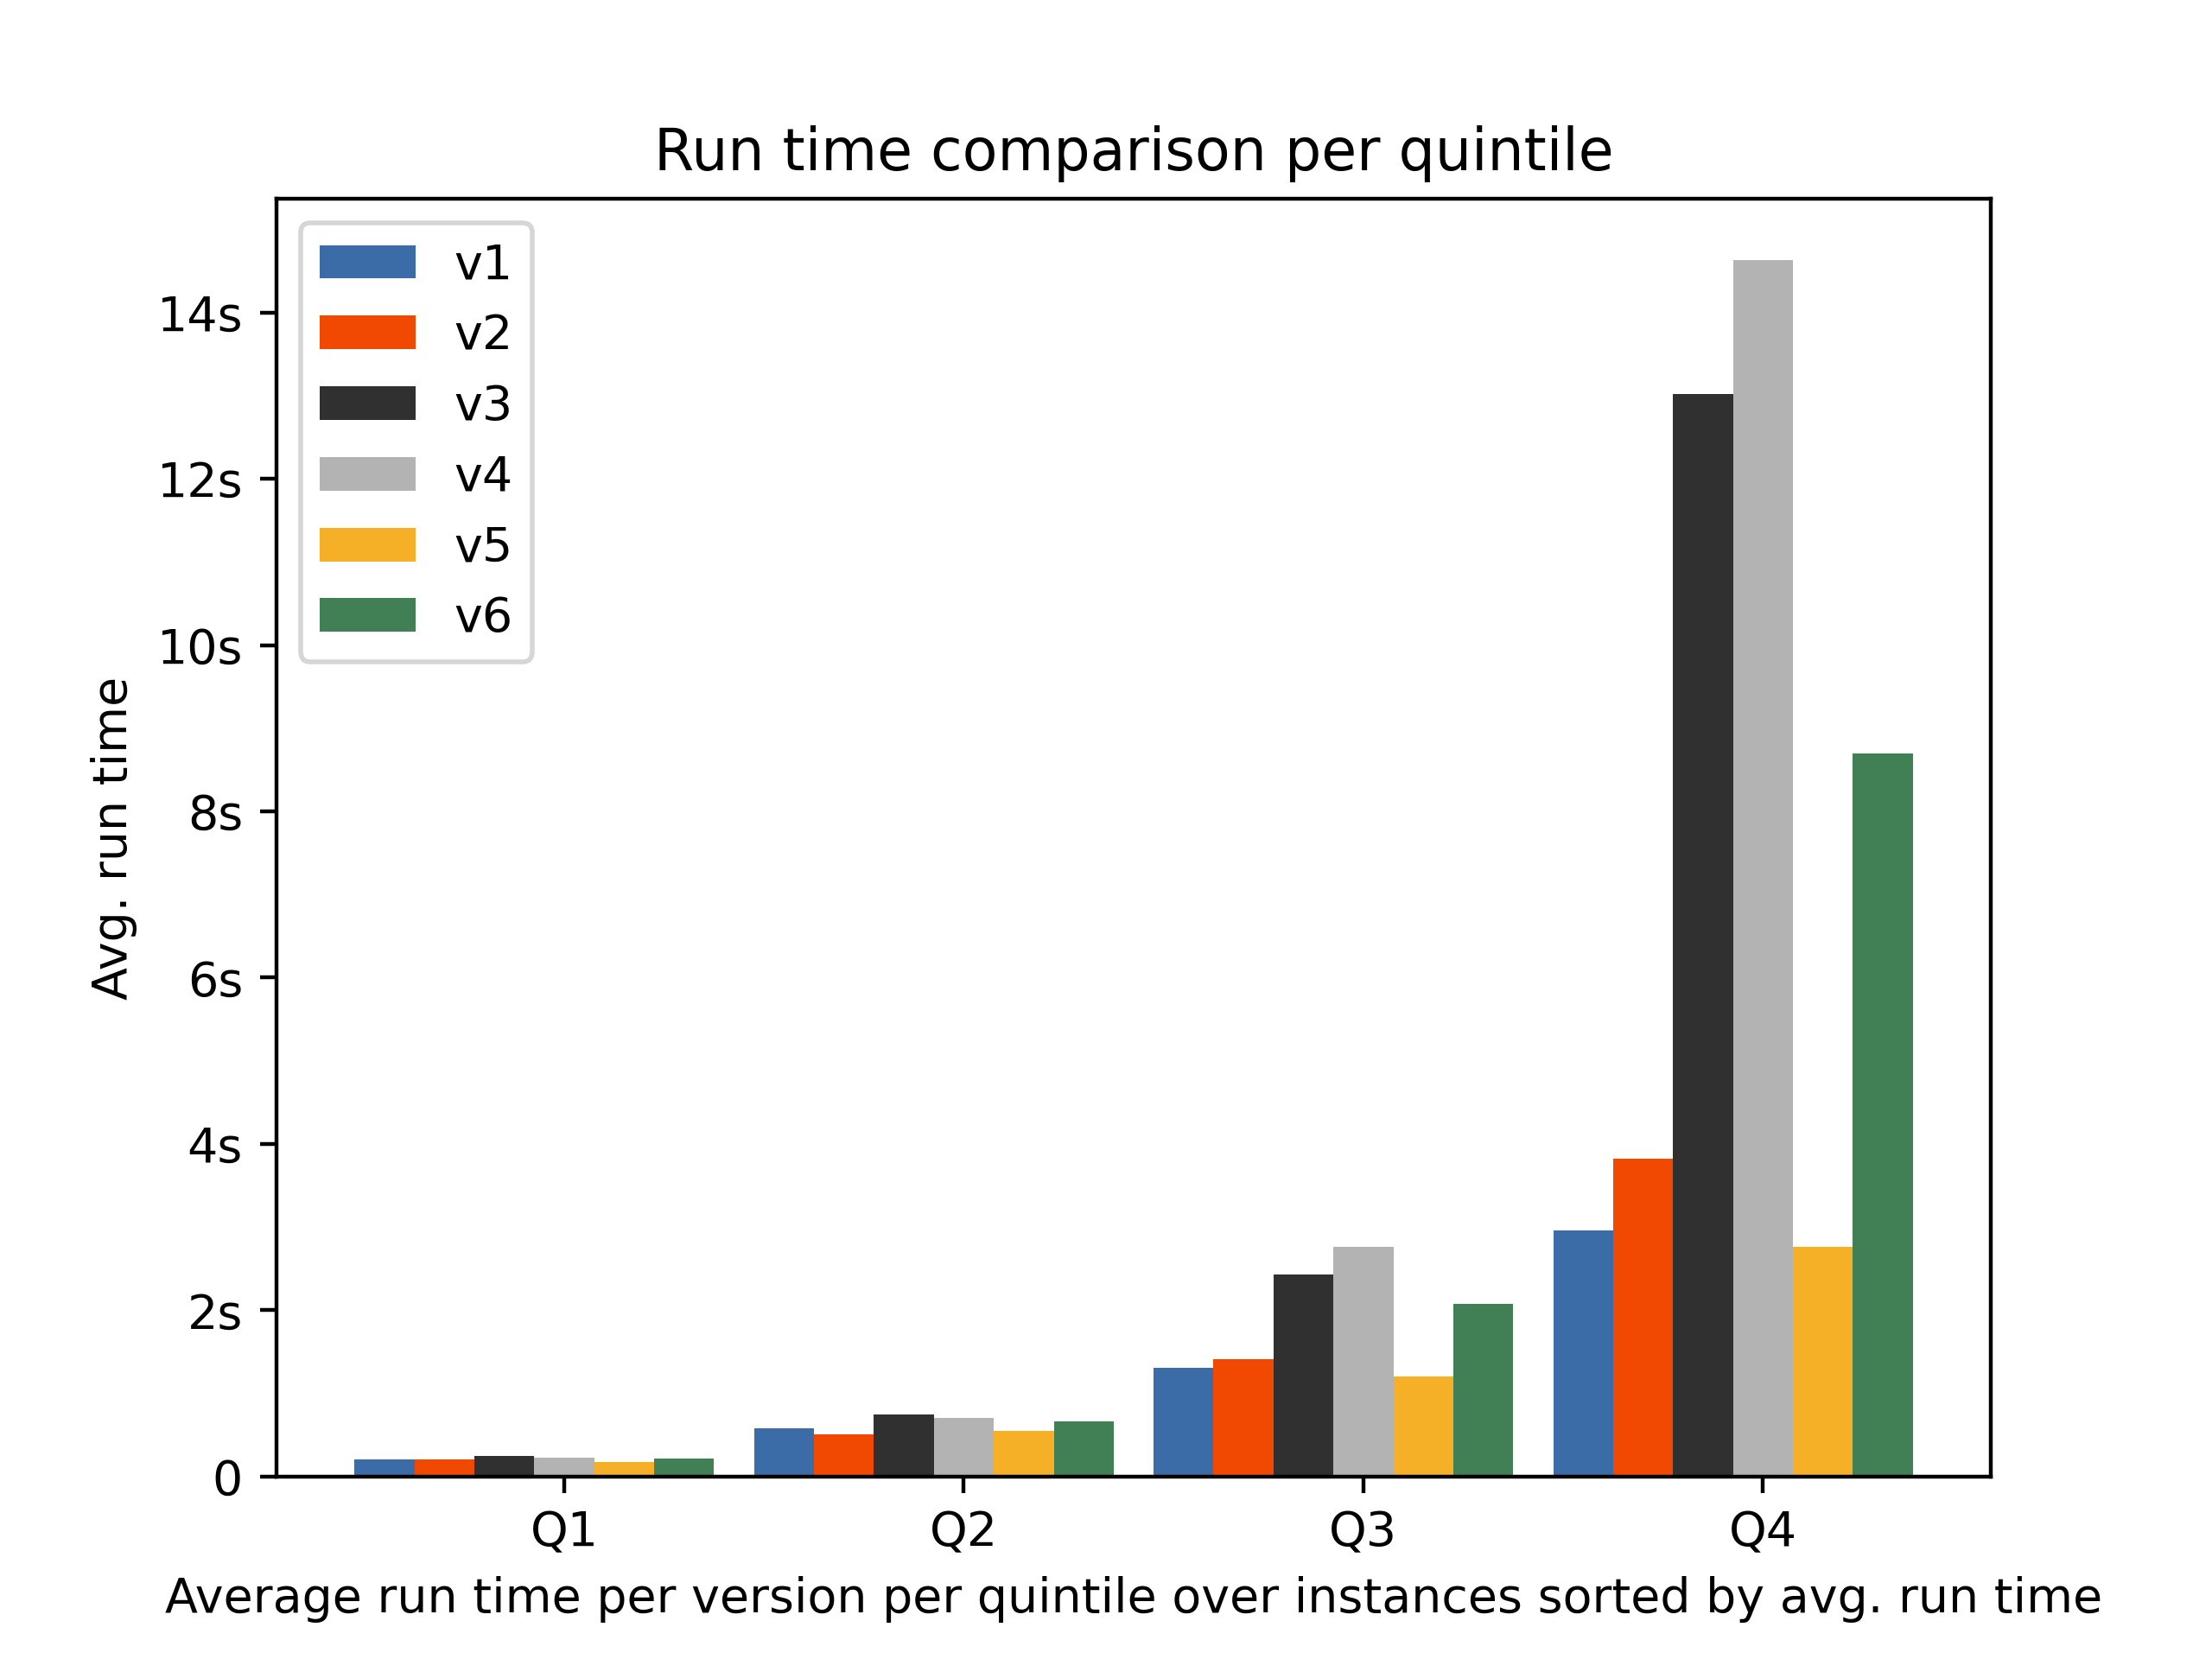
\includegraphics[width=10cm]{../resources/run_time_comparsion_by_quintile.png}
    \caption{Comparativa del tiempo de ejecución de todas las versiones en tiempo promedio para los cuatro primeros quintiles. El tiempo promedio considerado es acumulado sobre los quintiles anteriores. El último quintil está omitido dado que los tiempos de ejecución se disparan para algunas instancias.}
  \label{fig:firstfourquintiles}
\end{figure}

Considerando el tiempo de ejecución y el hecho de que no hubo incumplimientos en los chequeos de las soluciones, se perfila mejor las implementaciones que utilizan la segunda versión de formulación de $f_k$ y la función multiobjetivo 1, es decir la formulación v1. Sin embargo, previo a la elección final, decidimos solucionar el problema que causa diferencias en el valor de demanda transferida total y realizar la comparativa nuevamente.

Para solucionar la diferencia en demanda transferida cambiamos el valor del parámetro $\beta$ en (\ref{eq:multipleobj1}) de manera que se disminuye el efecto de las variables de $r_{kj}$ en la función objetivo de la formulación v1. El nuevo valor de $\beta$ es calculado para cada instancia y corresponde al factor mínimo entre los valores, para cada par origen-destino, que hace que el costo del camino más corto para dicho par sea menor a la menor cantidad de demanda que se transfiere de un punto de quiebre a otro. Es decir, se intenta encontrar un número que satisfaga: $\beta r_{kj} \leq min_{j \in J \setminus \{0\}} \{ P_{kj} - P_{k(j-1)} \},\; \forall r_{kj} \in [0, W_k]$.

Se ejecutaron nuevas pruebas comparando las tres versiones más rápidas: v1, v2 y v5. Esta vez se generaron 1000 nuevas instancias aleatorias con cuatro tecnologías lo que le da mayor complejidad. Nótese que si bien la v2 tiene incumplimientos estos no implican que las soluciones sean erróneas a los efectos de la demanda transferida total.

% La versión v1 modificada sobre las instancias de la primera ronda no genero soluciones con incumplimientos y su tiempo de ejecución promedio
% fue 10,31 segundos

\begin{table}[h!]
  \centering
  \begin{tabular}{ccc}
    \toprule
    Versión & Cant. Incump. & T. Promedio (s) \\
    \midrule
    v1 & 0   & 79.71   \\
    v2 & 119 & 282.11  \\
    v5 & 0   & 207.50  \\
    \bottomrule
  \end{tabular}
  \caption{Comparativa agregada de ejecuciones sobre la segunda ronda de instancias aleatorias sobre la red de Sioux-Falls.}\label{table:resumenreejecuciones}
\end{table}

\begin{figure}[h!]
  \centering
  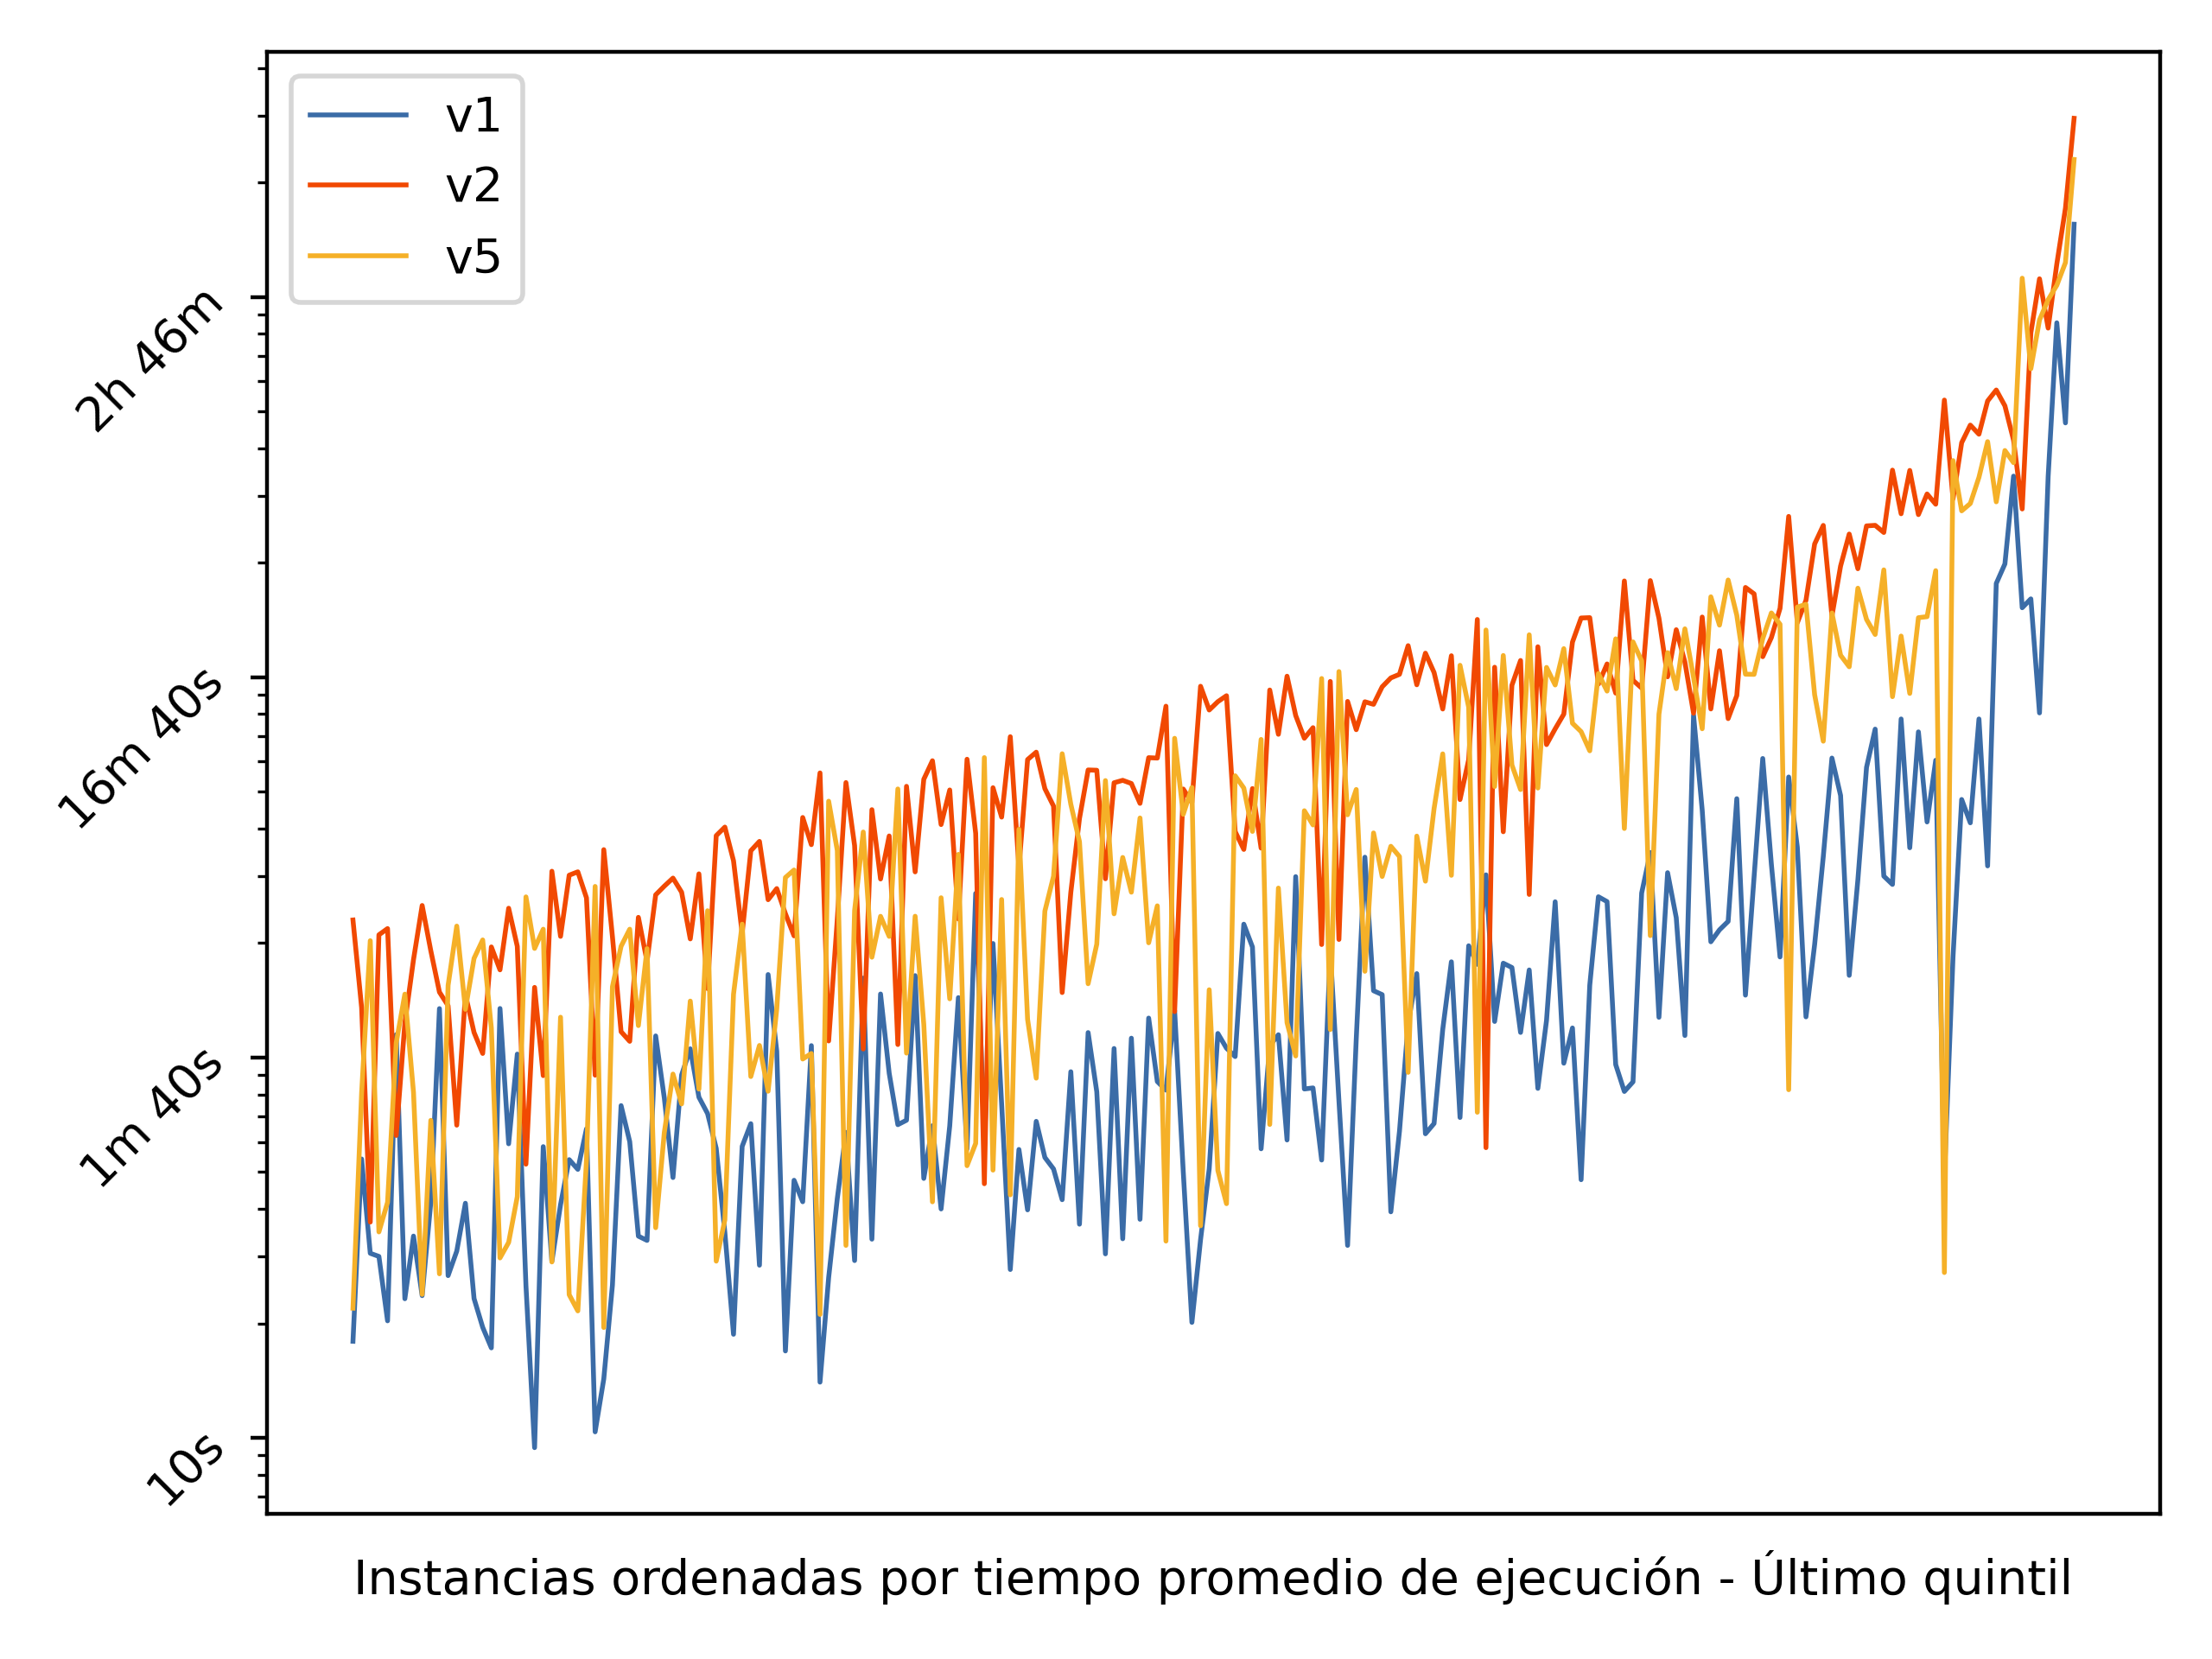
\includegraphics[width=10cm]{../resources/run_time_comparsion_rerun.png}
  \caption{Comparativa del tiempo de ejecución sobre la segunda ronda de instancias en los tres mejores modelos de la primera ronda. La escala es logarítmica en el eje de las ordenadas.} \label{fig:runtimecomparisonrerun}
\end{figure}

\begin{figure}[h!]
  \centering
  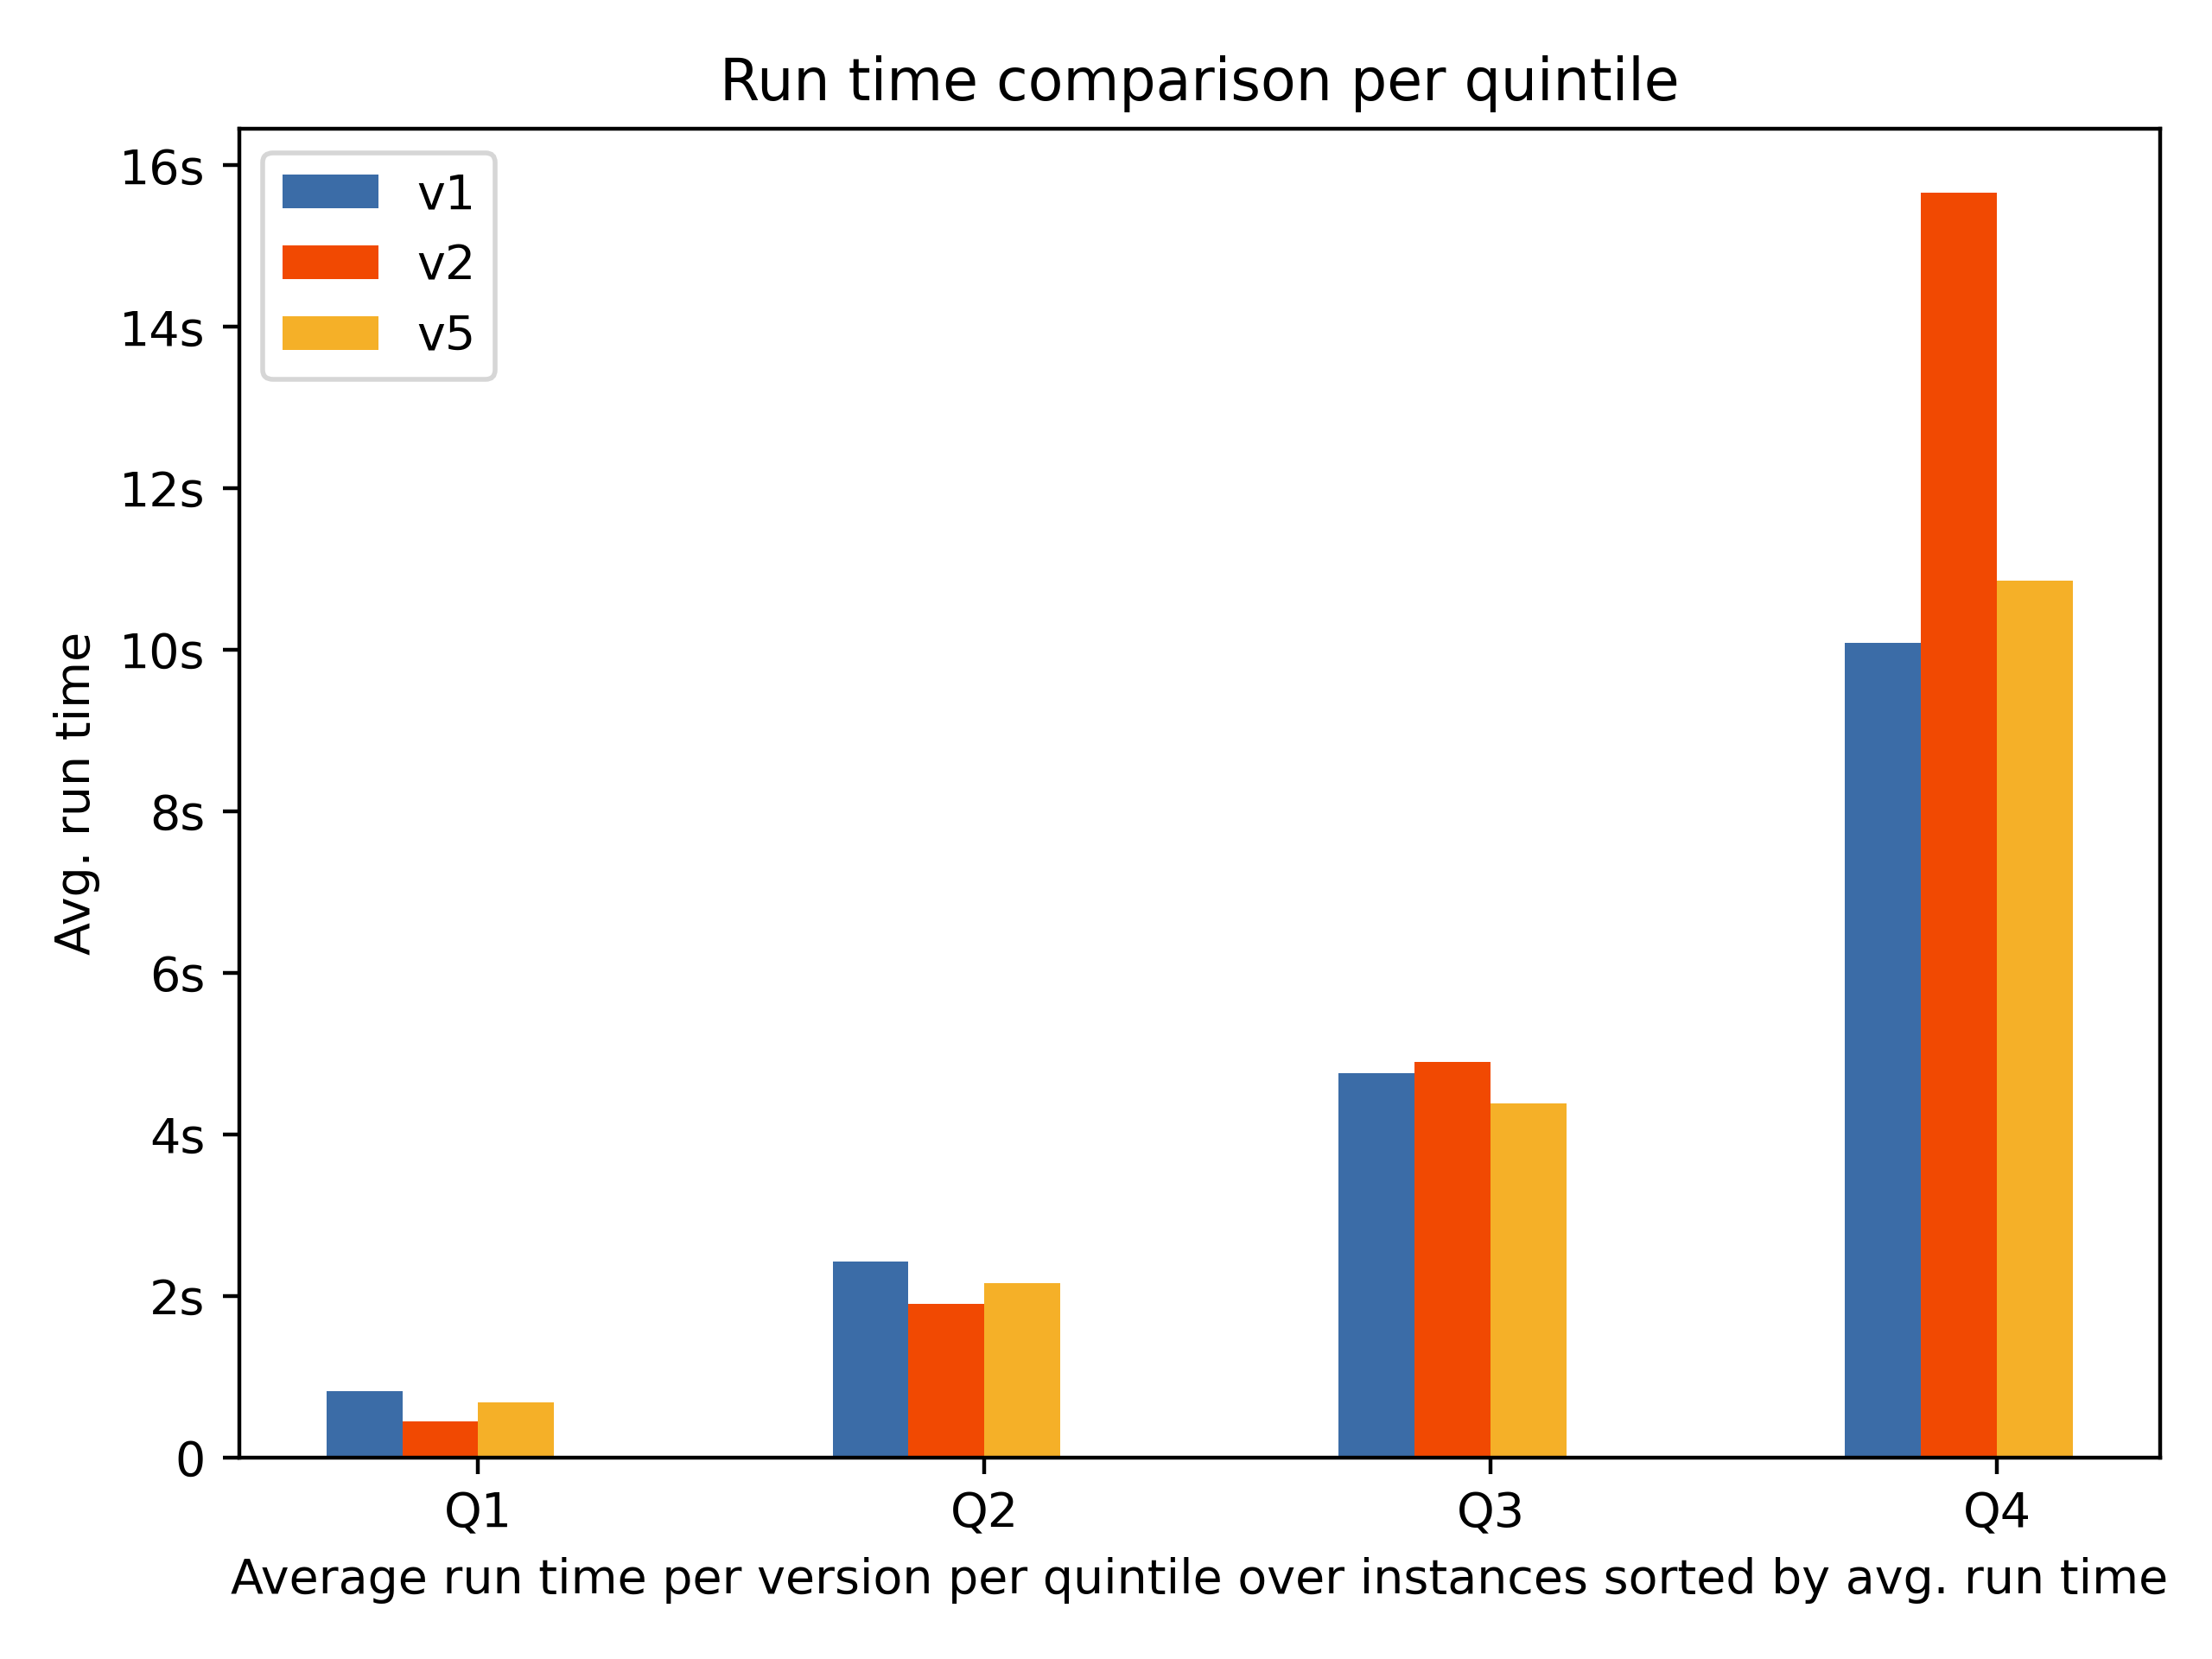
\includegraphics[width=10cm]{../resources/run_time_comparsion_by_quintile_rerun.png}
  \caption{Comparativa del tiempo de ejecución sobre la segunda ronda de instancias en los cuatro primeros quintiles. Las instancias fueron ordenadas por tiempo promedio de ejecución.} \label{fig:firstfourquintilesrerun}
\end{figure}

Los nuevos resultados se encuentran resumidos en la Tabla \ref{table:resumenreejecuciones}. En esta ronda de pruebas no detectamos diferencias en términos de la demanda transferida total y verificamos que la diferencia en la instancia problemática de la primera ronda fue solucionada. En términos de tiempo de ejecución, los resultados se encuentran en las Figuras \ref{fig:runtimecomparisonrerun} y \ref{fig:firstfourquintilesrerun}. Observamos que se mantiene el comportamiento de la ronda de pruebas anterior y la v1 sigue siendo más rápida. También observamos que el desempeño de v5 se degradó de peor manera. Dados los resultados, decidimos continuar el resto de este trabajo con la versión v1 de la formulación.
